\chapter{特征值与谱分解}
\label{chap:eigen-spectral-decomposition}
\label{chap:linear-analysis}
\label{chap:matrix-analysis}

第~\ref{chap:linear-representation}章说明，矩阵是线性映射在一组基下的坐标表示。对把空间映到自身的线性算子，输入和输出同时换成一组新基时，矩阵按相似关系$\bm B=\bm P^{-1}\bm A\bm P$改变（第~\ref{sec:ls-similarity}节），所以同一个作用有许多种矩阵写法。那里的例子中，算子$T(x_1,x_2)=(2x_1+x_2,3x_2)$在标准基下的矩阵有非零的非对角元，换到合适的基以后却成了对角矩阵：新基的两个方向在作用下只被伸缩，不被转向。

本章研究一般的表示问题：给定方阵，能否找到这样的方向？能找到多少？如果还要求新基保持长度和夹角，矩阵最多能化到多简单？这几个问题依次加强对基的要求，答案也依次收窄。

第~\ref{sec:ls-linear-operators}节寻找只被伸缩的方向，即特征向量，用特征多项式求出特征值，并说明它们不随基改变。第~\ref{sec:ls-matrix-powers}节判断特征向量何时多到足以组成一组基；这时矩阵相似于对角矩阵，矩阵幂化为特征值的乘方，但所用的特征基一般不正交。第~\ref{sec:ls-spectral-theory}节要求换基矩阵正交，证明能这样对角化的恰好是实对称矩阵，并把分解写成与基的选取无关的谱投影之和。第~\ref{sec:ls-general-square-spectrum}节处理一般方阵：允许复特征值以后，正交换基只能得到分块上三角的实Schur形，能化为分块对角形的恰好是正规矩阵。

本章用到第~\ref{chap:linear-operations}章的矩阵运算与行列式、第~\ref{chap:linear-representation}章的线性映射、换基与相似，以及第~\ref{chap:normed-inner-product-spaces}章的范数、内积、正交投影与正定矩阵。这里得到的谱定理是后面几章的共同工具：第~\ref{chap:singular-value-decomposition}章用它构造奇异值分解，第~\ref{chap:polar-decomposition}章用它开方，第~\ref{chap:condition-and-spectral-perturbation}章和第~\ref{chap:linear-recurrence-stability}章用特征值与谱半径分析扰动和反复作用。

% 第4章第1节：特征值与特征向量（特征方向、特征空间、特征多项式与Cayley--Hamilton定理、相似不变性、特征向量的线性无关性）。

\section{特征值与特征向量}
\label{sec:ls-linear-operators}

第~\ref{sec:ls-similarity}节的例子中，算子$T(x_1,x_2)=(2x_1+x_2,3x_2)$换到新基$\bm b_1'=\bm e_1$、$\bm b_2'=\bm e_1+\bm e_2$以后，矩阵成为对角矩阵$\operatorname{diag}(2,3)$，因为这两个基方向在作用下只被伸缩、不被转向。不过，那组基是事先给出、再加以验证的。

本节给出寻找这类方向的一般方法。特征向量的定义只说明要找什么；要系统地找出它们，需要把条件改写成特征多项式的根。求出的特征值还要与基无关，才是算子本身的性质；最后，不同特征值的特征向量线性无关，这为下一节用它们组成基作准备。

\subsection{线性作用中的特征方向}
\label{sec:ls-operator-eigenvectors}

第~\ref{sec:ls-linear-map-definition}节说明，线性算子$T:V\to V$总把原点留在原处，但一般会同时改变向量的长度和方向。我们要找的是这样的非零向量：作用以后仍落在原来那条过原点的直线上，只被伸长、缩短或反向。用等式表达，就是要求非零向量$\bm v\in V$与实数$\lambda$满足
\begin{equation}
T\bm v=\lambda\bm v,\qquad\bm v\neq\bm0.
\label{eq:matrix-analysis-eigenpair}
\end{equation}
这时称$\lambda$为$T$的\term{特征值}（eigenvalue），$\bm v$为属于$\lambda$的\term{特征向量}（eigenvector），$\bm v$所在的直线称为\term{特征方向}。

定义要求特征向量非零，因为零向量对任何$\lambda$都满足$T\bm0=\lambda\bm0$，不提供方向信息。特征值说明这条直线上发生了什么：$|\lambda|>1$时向量被拉长，$|\lambda|<1$时被缩短，$\lambda<0$时方向还被反过来；$\lambda=0$表示$T\bm v=\bm0$，即$\bm v$在$T$的核中。

在特征方向上，反复作用也最简单。第~\ref{sec:ls-operator-powers}节说明，算子可以与自身复合，得到$T^k$。对特征向量$\bm v$，由$T\bm v=\lambda\bm v$与线性性得$T^2\bm v=T(\lambda\bm v)=\lambda T\bm v=\lambda^2\bm v$，归纳即得$T^k\bm v=\lambda^k\bm v$。所以在这条直线上，$k$次作用化为数$\lambda$的$k$次乘方。

特征值是算子本身的性质，不依赖基的选取。取一组基$\mathcal B$后，式~\eqref{eq:matrix-analysis-eigenpair}的坐标形式是$[T]_{\mathcal B}[\bm v]_{\mathcal B}=\lambda[\bm v]_{\mathcal B}$。等式两侧分别是向量$T\bm v$与$\lambda\bm v$的坐标，而$\bm v\neq\bm0$当且仅当它的坐标非零。所以无论取哪组基，矩阵$[T]_{\mathcal B}$的特征值都恰好是$T$的特征值；换基只改变特征向量的坐标。

反过来，方阵也可以看作算子。对$n$阶方阵$\bm A$，它的特征值与特征向量指算子$\bm x\mapsto\bm A\bm x$的特征值与特征向量，即满足$\bm A\bm v=\lambda\bm v$、$\bm v\neq\bm0$的$\lambda$与$\bm v$。

回到开头的算子，可以逐个验证哪些方向是特征方向。
\begin{example}[验证特征向量]
\label{ex:ls-operator-eigenvector-check}
算子$T(x_1,x_2)=(2x_1+x_2,3x_2)$在标准基下的矩阵为
\[
 \bm A=\begin{bmatrix}2&1\\0&3\end{bmatrix}.
\]
我们看$\bm e_1$、$(1,1)^{\top}$与$\bm e_2$三个向量中哪些是特征向量。按定义，只需把每个向量乘以$\bm A$，看结果是否仍是原向量的倍数：
\[
\begin{gathered}
\bm A\bm e_1=\begin{bmatrix}2\\0\end{bmatrix}=2\bm e_1\\
\bm A\begin{bmatrix}1\\1\end{bmatrix}=\begin{bmatrix}3\\3\end{bmatrix}=3\begin{bmatrix}1\\1\end{bmatrix}\\
\bm A\bm e_2=\begin{bmatrix}1\\3\end{bmatrix}.
\end{gathered}
\]
前两个向量只被分别乘以$2$和$3$，所以$\bm e_1$与$(1,1)^{\top}$是特征向量，特征值分别为$2$和$3$；它们正是第~\ref{sec:ls-similarity}节新基的两个方向，这就解释了那组基为什么能把矩阵化成$\operatorname{diag}(2,3)$。$\bm e_2$则被送到$(1,3)^{\top}$，这不是$\bm e_2$的倍数，所以$\bm e_2$不是特征向量。
\end{example}
图~\ref{fig:ls-operator-eigenvectors}画出这个例子：两条特征方向上的向量作用后仍在原直线上，只是变长；其他方向上的向量被转开。
\begin{figure}[!htb]
  \centering
  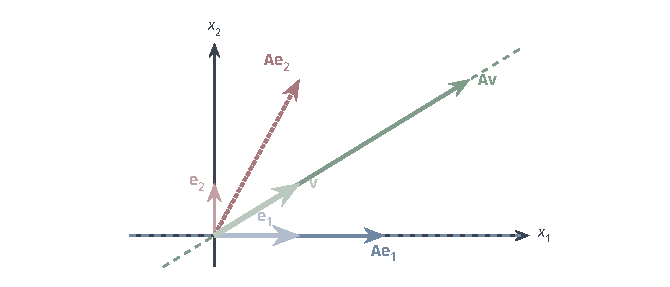
\includegraphics[width=112mm]{figures/00-shared/mathematical-preliminaries-upper/02-linear-spaces/tikz/comprehension-additions/operator-eigenvectors.pdf}
  \caption{特征向量只被伸缩、不被转向。算子$T(x_1,x_2)=(2x_1+x_2,3x_2)$在标准基下的矩阵为$\bm A=\left[\begin{smallmatrix}2&1\\0&3\end{smallmatrix}\right]$，它把$\bm e_1$送到$2\bm e_1$，把$\bm v=(1,1)^{\top}$送到$3\bm v$，二者都留在各自的虚线上；$\bm e_2$被送到$(1,3)^{\top}$，偏离了原来的直线，所以不是特征向量。}
  \label{fig:ls-operator-eigenvectors}
\end{figure}

并非每个算子都有实特征向量。下面的反例中，每个非零向量都被转离原来的直线。
\begin{example}[反例：平面旋转没有实特征向量]
\label{ex:ls-rotation-no-real-eigenvector}
考虑平面上逆时针旋转$90^\circ$的算子$R(x_1,x_2)=(-x_2,x_1)$。直观上，每个非零向量都被转过直角，不可能留在原来的直线上；下面用方程确认这一点。设实数$\lambda$与向量$(x_1,x_2)$满足$R(x_1,x_2)=\lambda(x_1,x_2)$，按分量写出就是
\[
 \begin{gathered}
-x_2=\lambda x_1\\
x_1=\lambda x_2 .
 \end{gathered}
\]
把第二式代入第一式得$-x_2=\lambda^2x_2$，即$(1+\lambda^2)x_2=0$。由于$1+\lambda^2>0$，只能$x_2=0$，进而$x_1=\lambda x_2=0$。可见无论取哪个实数$\lambda$，满足等式的都只有零向量，所以$R$既没有实特征值，也没有实特征向量。
\end{example}

\subsection{特征空间与不变子空间}

同一个特征值可以对应不止一条特征方向，所以应把它们放在一起考察。固定特征值$\lambda$，满足$T\bm v=\lambda\bm v$的全部向量连同零向量组成集合$\ker(T-\lambda\,\operatorname{id}_V)$，称为$\lambda$的\term{特征空间}（eigenspace）。它是一个线性映射的核，因而是子空间。

例如$\bm I_2$的每个非零向量都是属于$1$的特征向量，特征空间是整个平面；而示例~\ref{ex:ls-operator-eigenvector-check}中属于$2$的特征空间只是$\bm e_1$所在的直线，因为$\bm A-2\bm I=\left[\begin{smallmatrix}0&1\\0&1\end{smallmatrix}\right]$的核由第二坐标为零的向量组成。

特征空间是一类更一般的子空间的特例。若子空间$S$满足$T(S)\subseteq S$，就称$S$为$T$的\term{不变子空间}（invariant subspace）。这时作用不会把$S$中的向量带出$S$，可以把$T$限制在$S$上单独研究。特征空间中的向量只被乘以$\lambda$，仍留在其中，所以特征空间是不变子空间。

一维不变子空间恰好就是特征方向。若$\bm v\neq\bm0$且$\operatorname{span}\{\bm v\}$不变，则$T\bm v$落在这条直线上，是$\bm v$的倍数；反之，若$T\bm v=\lambda\bm v$，则$T(c\bm v)=\lambda c\bm v$仍在这条直线上。高于一维的不变子空间却未必含有特征方向：整个平面对$90^\circ$旋转不变，而示例~\ref{ex:ls-rotation-no-real-eigenvector}说明其中没有一条特征方向。这样的二维不变子空间对应一对共轭的复特征值（第~\ref{sec:ls-general-square-spectrum}节）。

\subsection{特征多项式}
\label{sec:ls-characteristic-polynomial}

示例~\ref{ex:ls-operator-eigenvector-check}中的特征向量是先猜出、再验证的。要系统地求出全部特征值，可以把特征值的条件改写成矩阵不可逆。对$n$阶方阵$\bm A$，$\lambda$是特征值，当且仅当齐次方程$(\bm A-\lambda\bm I)\bm v=\bm0$有非零解，即$\ker(\bm A-\lambda\bm I)\neq\{\bm0\}$。由第~\ref{sec:ls-injective-surjective-invertible}节的等价条件，这又等价于$\operatorname{rank}(\bm A-\lambda\bm I)<n$，也等价于$\bm A-\lambda\bm I$不可逆。

不可逆又等价于行列式为零，这一步用到第~\ref{sec:ls-determinant-properties}节的两条性质。若方阵$\bm M$可逆，乘法性给出$\det\bm M\det(\bm M^{-1})=\det\bm I=1$，故$\det\bm M\neq0$；反之若$\det\bm M\neq0$，古典伴随恒等式说明$\operatorname{adj}(\bm M)/\det\bm M$就是$\bm M$的逆。所以$\lambda$是$\bm A$的特征值，当且仅当$\det(\bm A-\lambda\bm I)=0$。

这也解释了第~\ref{sec:ls-similarity-properties}节的一个相似不变量。那里把每个$\operatorname{rank}(\bm A-c\bm I)$都列为相似不变量；现在可以看出，使这个秩小于$n$的数$c$恰好就是特征值。

把这个条件写成首项系数为$1$的多项式更方便。由于$\det(\lambda\bm I-\bm A)=(-1)^n\det(\bm A-\lambda\bm I)$，二者同时为零。定义
\begin{equation}
 p_{\bm A}(z)=\det(z\bm I-\bm A),
 \label{eq:matrix-analysis-characteristic-polynomial}
\end{equation}
称为\term{特征多项式}（characteristic polynomial），就得到：$\bm A$的实特征值恰为$p_{\bm A}$的实根。

再看$p_{\bm A}$的次数。在行列式的排列展开中，对角线一项是$\prod_i(z-a_{i,i})$；其余每一项至少有两个因子取自非对角位置，含$z$的因子至多$n-2$个。所以只有对角线一项含$z^n$，$p_{\bm A}$是首项系数为$1$的$n$次实多项式，至多有$n$个不同的根。求出一个特征值$\lambda$以后，再解齐次方程$(\bm A-\lambda\bm I)\bm v=\bm0$，就得到它的特征空间。

用特征多项式可以重新求出前面两个例子的特征值，不必再猜测特征向量。
\begin{example}[用特征多项式求特征值]
\label{ex:ls-characteristic-polynomial-two-by-two}
回到示例~\ref{ex:ls-operator-eigenvector-check}的矩阵$\bm A$，以及示例~\ref{ex:ls-rotation-no-real-eigenvector}中旋转在标准基下的矩阵$\bm R$：
\[
 \bm A=\begin{bmatrix}2&1\\0&3\end{bmatrix},\qquad
 \bm R=\begin{bmatrix}0&-1\\1&0\end{bmatrix}.
\]
这一次不猜特征向量，而是直接计算$\det(z\bm I-\bm A)$与$\det(z\bm I-\bm R)$：
\[
 \begin{aligned}
 p_{\bm A}(z)&=\det\begin{bmatrix}z-2&-1\\0&z-3\end{bmatrix}=(z-2)(z-3),\\
 p_{\bm R}(z)&=\det\begin{bmatrix}z&1\\-1&z\end{bmatrix}=z^2+1 .
 \end{aligned}
\]
$p_{\bm A}$的两个根$2$与$3$正是示例~\ref{ex:ls-operator-eigenvector-check}中两条特征方向上的伸缩倍数，而且这里不需要事先知道那两条方向。$z^2+1$对任何实数$z$都为正，没有实根，所以$\bm R$没有实特征值，与示例~\ref{ex:ls-rotation-no-real-eigenvector}直接解方程的结论一致。
\end{example}
$\bm A$的情形可以推广到任意三角矩阵：三角矩阵$\bm A$的$z\bm I-\bm A$仍是三角矩阵，行列式是对角元之积$\prod_i(z-a_{i,i})$，所以三角矩阵的特征值就是它的对角元。

特征多项式在每个特征值处取零。把矩阵本身代入特征多项式，结果是零矩阵。这里的代入是指把多项式中的$z^j$换成$\bm A^j$，常数项$c_0$换成$c_0\bm I$。先在一个例子中验证。
\begin{example}[把矩阵代入它的特征多项式]
\label{ex:ls-cayley-hamilton-two-by-two}
仍取
\[
 \bm A=\begin{bmatrix}2&1\\0&3\end{bmatrix}.
\]
由示例~\ref{ex:ls-characteristic-polynomial-two-by-two}，$p_{\bm A}(z)=(z-2)(z-3)=z^2-5z+6$。把$z^2$换成$\bm A^2$、$z$换成$\bm A$、常数$6$换成$6\bm I$，需要先算出$\bm A^2$，再逐个元素合并：
\[
\begin{gathered}
\bm A^2=\begin{bmatrix}4&5\\0&9\end{bmatrix}\\
\bm A^2-5\bm A+6\bm I
 =\begin{bmatrix}4-10+6&5-5+0\\0&9-15+6\end{bmatrix}
 =\bm0 .
\end{gathered}
\]
四个元素全部抵消，$p_{\bm A}(\bm A)$是零矩阵。两个对角元分别是$p_{\bm A}(2)$与$p_{\bm A}(3)$，为零是因为$2,3$是特征值；右上角的抵消则来自$\bm A^2$与$5\bm A$的非对角元恰好相等，单看特征值处取零并不能预见。
\end{example}
这一结论对每个方阵都成立。
\begin{theorem}[Cayley--Hamilton定理]
\label{thm:ls-cayley-hamilton}
设$n$阶方阵$\bm A$的特征多项式为$p_{\bm A}(z)=z^n+c_{n-1}z^{n-1}+\cdots+c_0$，则
\[
 p_{\bm A}(\bm A)
 =\bm A^n+c_{n-1}\bm A^{n-1}+\cdots+c_1\bm A+c_0\bm I=\bm0.
\]
\end{theorem}
\begin{proof}
证明的工具是第~\ref{sec:ls-det-cofactor-adjugate}节的古典伴随恒等式（定理~\ref{thm:ls-adjugate-identity}）$\bm M\operatorname{adj}(\bm M)=\det(\bm M)\bm I$。令$\bm M=z\bm I-\bm A$，得
\[
 (z\bm I-\bm A)\operatorname{adj}(z\bm I-\bm A)=p_{\bm A}(z)\bm I .
\]
$\operatorname{adj}(z\bm I-\bm A)$的每个元素都是$z\bm I-\bm A$的一个带符号的$n-1$阶余子式，它是$z$的多项式，次数不超过$n-1$。按$z$的幂次整理，可以写成$\operatorname{adj}(z\bm I-\bm A)=\sum_{j=0}^{n-1}z^j\bm B_j$，其中$\bm B_j$是不含$z$的常数矩阵。

代入上式，左边为$\sum_jz^{j+1}\bm B_j-\sum_jz^j\bm A\bm B_j$。两边每个元素都是$z$的多项式，且对所有实数$z$相等，所以同次项的系数相等。记$c_n=1$，比较$z$的各次幂系数：
\[
 \begin{aligned}
 &z^n: &&\bm B_{n-1}=\bm I;\\
 &z^j\ (1\leq j\leq n-1): &&\bm B_{j-1}-\bm A\bm B_j=c_j\bm I;\\
 &z^0: &&-\bm A\bm B_0=c_0\bm I .
 \end{aligned}
\]
把$z^j$项的等式左乘$\bm A^j$（$j=0,\ldots,n$）后相加。右边恰为$\sum_jc_j\bm A^j=p_{\bm A}(\bm A)$；左边为
\[
 \bm A^n\bm B_{n-1}+\sum_{j=1}^{n-1}\bigl(\bm A^j\bm B_{j-1}-\bm A^{j+1}\bm B_j\bigr)-\bm A\bm B_0 ,
\]
其中相邻项逐对相消，总和为零。
\end{proof}
证明只用到行列式与古典伴随，既不需要先求出特征值，也不要求$p_{\bm A}$有实根。

由定理可以推出，矩阵的高次幂都能由低次幂表示。
\begin{theorem}[高次幂的降次]
\label{thm:ls-power-reduction}
设$\bm A$为$n$阶方阵，则对每个整数$k\geq0$，
\[
 \bm A^k\in\operatorname{span}\{\bm I,\bm A,\ldots,\bm A^{n-1}\}.
\]
因而对任意向量$\bm g$与$k\geq0$，
\[
 \bm A^k\bm g\in\operatorname{span}\{\bm g,\bm A\bm g,\ldots,\bm A^{n-1}\bm g\},
\]
前$k$项$\bm g,\ldots,\bm A^{k-1}\bm g$张成的子空间在$k\geq n$时不再增大。
\end{theorem}
\begin{proof}
记$\mathcal P=\operatorname{span}\{\bm I,\bm A,\ldots,\bm A^{n-1}\}$。$k<n$时结论显然。对$k\geq n$归纳。$k=n$时，由定理~\ref{thm:ls-cayley-hamilton}，
\[
 \bm A^n=-\sum_{j=0}^{n-1}c_j\bm A^j\in\mathcal P .
\]
设$\bm A^k=\sum_{j=0}^{n-1}d_j\bm A^j\in\mathcal P$。两边左乘$\bm A$，得
\[
 \bm A^{k+1}=\sum_{j=0}^{n-2}d_j\bm A^{j+1}+d_{n-1}\bm A^n .
\]
右端第一个和属于$\mathcal P$，$\bm A^n$也属于$\mathcal P$，所以$\bm A^{k+1}\in\mathcal P$。

对向量$\bm g$，把$\bm A^k=\sum_jd_j\bm A^j$作用于$\bm g$，即得$\bm A^k\bm g=\sum_{j=0}^{n-1}d_j\bm A^j\bm g$。于是$k\geq n$时新加入的向量$\bm A^{k-1}\bm g$已在前$n$个向量张成的子空间中，子空间不再增大。
\end{proof}
所以序列$\bm g,\bm A\bm g,\bm A^2\bm g,\ldots$张成的子空间至多是$n$维的，并且由前$n$项决定。第~\ref{chap:matrix-equations}章判断Sylvester方程何时有唯一解，第~\ref{chap:krylov-methods}章研究Krylov子空间方法时，都要用到这一点。

回到特征值本身。同一个特征值可以是特征多项式的重根，这时要区分两种“个数”。根$\lambda$在$p_{\bm A}$中的重数称为\term{代数重数}（algebraic multiplicity），特征空间的维数$\dim\ker(\bm A-\lambda\bm I)$称为\term{几何重数}（geometric multiplicity）。下面的例子说明二者可以不同。
\begin{example}[代数重数大于几何重数]
\label{ex:ls-multiplicity-gap}
取
\[
 \bm J=\begin{bmatrix}0.8&1\\0&0.8\end{bmatrix}.
\]
它是上三角矩阵，特征多项式为$p_{\bm J}(z)=(z-0.8)^2$，所以唯一的特征值$0.8$是二重根，代数重数为$2$。要知道几何重数，还得解出特征空间：
\[
\begin{gathered}
\bm J-0.8\bm I=\begin{bmatrix}0&1\\0&0\end{bmatrix}\\
(\bm J-0.8\bm I)\begin{bmatrix}x_1\\x_2\end{bmatrix}=\begin{bmatrix}x_2\\0\end{bmatrix},
\end{gathered}
\]
它为零当且仅当$x_2=0$，所以特征空间只是$(1,0)^{\top}$所在的直线，几何重数为$1$。特征多项式把$0.8$数了两次，特征方向却只有一条；右上角的$1$正是使第二条特征方向消失的原因。
\end{example}
两种重数的一般关系，以及它们怎样决定能否找到由特征向量组成的基，在第~\ref{sec:ls-matrix-powers}节讨论。对一般的算子$T$，可以取任一组基把它写成矩阵，再求特征多项式与两种重数。下一小节说明，结果不依赖基的选取。

\subsection{相似变换与谱的不变性}
\label{sec:ls-eigen-similarity-invariance}

第~\ref{sec:ls-similarity-properties}节列出了相似保持的量：秩、零空间的维数、每个$\operatorname{rank}(\bm A-c\bm I)$，以及行列式与迹。本小节说明，特征值、特征多项式与两种重数也是相似不变量，因此它们属于算子本身；再说明迹与行列式怎样由特征值读出，最后指出这些不变量只能否定相似。

\paragraph{特征值、特征空间与特征多项式}
下面的定理把这些不变性一并写出。

\begin{theorem}[谱的相似不变性]
\label{thm:ls-spectrum-similarity-invariance}
设$\bm B=\bm P^{-1}\bm A\bm P$，$\bm P$可逆，则：
\begin{enumerate}
 \item $\bm A$与$\bm B$的特征值相同；若$\bm A\bm v=\lambda\bm v$，则$\bm B(\bm P^{-1}\bm v)=\lambda\bm P^{-1}\bm v$，且$\ker(\bm B-\lambda\bm I)=\bm P^{-1}\ker(\bm A-\lambda\bm I)$，所以每个特征值的几何重数相同；
 \item $p_{\bm B}=p_{\bm A}$，所以每个特征值的代数重数相同。
\end{enumerate}
\end{theorem}
\begin{proof}
第一条。若$\bm A\bm v=\lambda\bm v$且$\bm v\neq\bm0$，则
\[
 \bm B(\bm P^{-1}\bm v)=\bm P^{-1}\bm A\bm P\bm P^{-1}\bm v=\bm P^{-1}\bm A\bm v=\lambda\bm P^{-1}\bm v .
\]
$\bm P$可逆保证$\bm P^{-1}\bm v\neq\bm0$，所以$\lambda$也是$\bm B$的特征值；交换$\bm A,\bm B$的角色即得反向结论。同样的计算说明$\bm P^{-1}$把$\ker(\bm A-\lambda\bm I)$映入$\ker(\bm B-\lambda\bm I)$，交换角色可知$\bm P$把后者映入前者，所以$\ker(\bm B-\lambda\bm I)=\bm P^{-1}\ker(\bm A-\lambda\bm I)$。可逆矩阵把子空间映成同维数的子空间，所以几何重数相同。这一结论也可以由式~\eqref{eq:ls-similarity-shifted-rank}取$c=\lambda$、再用秩零度定理换成核的维数得到。

第二条。由$z\bm I=\bm P^{-1}(z\bm I)\bm P$与第~\ref{sec:ls-similarity-properties}节的恒等式$\det(\bm P^{-1}\bm M\bm P)=\det\bm M$，
\[
 p_{\bm B}(z)=\det(z\bm I-\bm P^{-1}\bm A\bm P)=\det\bigl(\bm P^{-1}(z\bm I-\bm A)\bm P\bigr)=p_{\bm A}(z).
\]
\end{proof}
所以算子的特征值、特征多项式与两种重数都可以用任意一组基下的矩阵计算。

\paragraph{特征多项式的系数}
行列式与迹也是相似不变量，这可以由定理~\ref{thm:ls-spectrum-similarity-invariance}解释：它们就是$p_{\bm A}$的两个系数，至多差一个符号。
\begin{theorem}[迹、行列式与特征值]
\label{thm:ls-trace-det-eigenvalues}
设$\bm A$为$n$阶方阵，则
\[
 p_{\bm A}(z)=z^n-(\operatorname{tr}\bm A)\,z^{n-1}+\cdots+(-1)^n\det\bm A .
\]
若$p_{\bm A}(z)=\prod_{i=1}^n(z-\lambda_i)$分解为实一次因子之积，其中每个特征值按代数重数重复列出，则
\[
 \operatorname{tr}\bm A=\sum_{i=1}^n\lambda_i,\qquad\det\bm A=\prod_{i=1}^n\lambda_i .
\]
\end{theorem}
\begin{proof}
令$z=0$，得常数项$p_{\bm A}(0)=\det(-\bm A)=(-1)^n\det\bm A$。再看$z^{n-1}$的系数。第~\ref{sec:ls-characteristic-polynomial}节已经指出，排列展开中除对角线一项外，每一项含$z$的因子至多$n-2$个；所以$z^{n-1}$只来自$\prod_i(z-a_{i,i})$，系数为$-\sum_ia_{i,i}=-\operatorname{tr}\bm A$。若$p_{\bm A}=\prod_i(z-\lambda_i)$，展开右端，$z^{n-1}$的系数为$-\sum_i\lambda_i$，常数项为$(-1)^n\prod_i\lambda_i$，与上面比较即得两个等式。
\end{proof}
例如示例~\ref{ex:ls-operator-eigenvector-check}的$\bm A$有$\operatorname{tr}\bm A=5=2+3$，$\det\bm A=6=2\cdot3$。第~\ref{sec:ls-general-square-spectrum}节把特征多项式的复根也算作特征值以后，这两个等式对每个方阵都成立。

\paragraph{相似不变量只能否定相似}
相似不变量只能用来否定相似：某个相似不变量不同，两个矩阵就不相似；不变量全部相同，两个矩阵却未必相似。第~\ref{sec:ls-similarity-conditions}节比较过$\bm I_2$与$\left[\begin{smallmatrix}1&1\\0&1\end{smallmatrix}\right]$，下面用特征值的语言重新说明二者为什么不相似。
\begin{example}[反例：特征多项式相同而不相似]
\label{ex:ls-same-charpoly-not-similar}
比较$\bm I_2$与
\[
 \bm J_1=\begin{bmatrix}1&1\\0&1\end{bmatrix}.
\]
二者都是上三角矩阵，对角元都是$1$，所以$p_{\bm I_2}(z)=p_{\bm J_1}(z)=(z-1)^2$，特征值$1$的代数重数都是$2$。仅凭特征多项式无法把它们区分开，于是转而比较特征空间：
\[
\begin{gathered}
\bm I_2-\bm I_2=\bm0\\
\bm J_1-\bm I_2=\begin{bmatrix}0&1\\0&0\end{bmatrix},
\end{gathered}
\]
前者的核是整个平面，后者的核只是$(1,0)^{\top}$所在的直线，几何重数分别为$2$与$1$。由定理~\ref{thm:ls-spectrum-similarity-invariance}，相似矩阵的几何重数必须相同，所以二者不相似，尽管它们的特征多项式完全一样。
\end{example}
所以特征多项式相同只是相似的必要条件。比较各特征值的几何重数是更细的必要条件，但一般仍不足以判定相似；完整的相似分类需要Jordan标准形，本书不展开。

\subsection{特征向量的线性无关性}
\label{sec:ls-eigenvector-independence}

要用特征方向组成一组基，先要知道不同特征值的特征向量彼此不会重复。本小节先证明它们线性无关，再推出各特征空间之和是直和。

\paragraph{特征向量的线性无关}
设想两条特征方向属于不同的特征值。若其中一条落在另一条上，同一个向量就会被乘以两个不同的倍数，这不可能。下面的定理把这一观察推广到任意多个特征值。
\begin{theorem}[不同特征值的特征向量线性无关]
\label{thm:ls-distinct-eigenvectors-independent}
设$\bm v_1,\ldots,\bm v_r$分别是$T$属于互不相同的特征值$\lambda_1,\ldots,\lambda_r$的特征向量，则$\bm v_1,\ldots,\bm v_r$线性无关。特别地，$n$维空间上的算子至多有$n$个不同的特征值。
\end{theorem}
\begin{proof}
假设它们线性相关。在所有非平凡的线性依赖中取项数最少的一个，重新编号后记为$\sum_{j=1}^s c_j\bm v_j=\bm0$，其中各$c_j\neq0$；单个特征向量非零，不能单独构成依赖，所以$s\geq2$。两边作用$T-\lambda_1\operatorname{id}_V$：第一项变为零，其余各项变为$c_j(\lambda_j-\lambda_1)\bm v_j$。特征值互不相同，这些系数仍非零，于是得到一个只有$s-1$项的非平凡依赖，与$s$最少矛盾。$n$维空间中线性无关的向量至多$n$个，所以不同特征值至多$n$个。
\end{proof}
这一上界与特征多项式的次数给出的上界一致。

\paragraph{特征空间的直和}
同一个特征值可以有多维的特征空间。从每个特征空间各取一组基，合在一起是否仍线性无关？下面的定理给出肯定回答。
\begin{theorem}[特征空间之和是直和]
\label{thm:ls-eigenspaces-direct-sum}
设$\lambda_1,\ldots,\lambda_r$是$T$的互不相同的特征值，$E_i=\ker(T-\lambda_i\operatorname{id}_V)$。则和$E_1+\cdots+E_r$是直和；把各$E_i$的基合在一起，仍线性无关，因而$\dim(E_1+\cdots+E_r)=\sum_i\dim E_i$。
\end{theorem}
\begin{proof}
设$\bm w_1+\cdots+\bm w_r=\bm0$，$\bm w_i\in E_i$。其中非零的$\bm w_i$是属于不同特征值的特征向量，由定理~\ref{thm:ls-distinct-eigenvectors-independent}线性无关，不能相加为零，所以每个$\bm w_i=\bm0$，和是直和。把各$E_i$的基合在一起，它们的任一线性组合都可以按特征值分组写成$\sum_i\bm w_i$；若组合为零，则每个$\bm w_i=\bm0$，而每组基本身线性无关，所以全部系数为零。
\end{proof}

例如示例~\ref{ex:ls-operator-eigenvector-check}中的$\bm e_1$与$(1,1)^{\top}$属于不同的特征值$2$与$3$，不必另行验证，它们自动线性无关，在平面上组成一组基。

回顾本节：被算子只伸缩的方向是特征方向，伸缩倍数是特征值。特征值是特征多项式的实根，求出特征值后解齐次方程即得特征空间。特征值、特征多项式和两种重数都不随基改变，属于算子本身。

属于不同特征值的特征向量线性无关，所以$n$维空间上的算子至多有$n$个不同特征值。此外，Cayley--Hamilton定理说明$p_{\bm A}(\bm A)=\bm0$，由此$\bm A$的高次幂都能用$\bm I,\bm A,\ldots,\bm A^{n-1}$表示（定理~\ref{thm:ls-power-reduction}）。特征向量什么时候多到足以组成一组基，是下一节的对角化问题。

% 第4章第2节：对角化（特征基下的矩阵与幂、可对角化的判别及不能对角化的情形、计算步骤与算例）。

\section{对角化}
\label{sec:ls-matrix-powers}
\label{sec:ch06-powers-spectrum}

上一节找到了被算子只伸缩的方向，并证明属于不同特征值的特征向量线性无关。本节考察这些方向足以组成一组基的情形。先看这时矩阵和矩阵幂变成什么样，由此明白这种基为什么值得寻找；再给出它存在的条件，最后整理计算步骤。

本节的换基矩阵只要求可逆，各列不必互相垂直；要求正交换基的情形留给下一节。

\subsection{特征向量基下的矩阵表示}
\label{sec:matrix-analysis-spectrum}

设$\bm v_1,\ldots,\bm v_n$是由算子$T$的特征向量组成的基，$T\bm v_j=\lambda_j\bm v_j$。按第~\ref{sec:ls-map-representation}节的约定，$T$在这组基下的矩阵的第$j$列是$T\bm v_j=\lambda_j\bm v_j$的坐标，即第$j$个位置为$\lambda_j$、其余位置为零。所以这个矩阵在主对角线以外全为零，每个基方向被独立地伸缩。

示例~\ref{ex:ls-operator-eigenvector-check}中的$(\bm e_1,(1,1)^{\top})$就是这样一组基。换到这组基，正是第~\ref{sec:ls-similarity}节的相似变换$\bm P^{-1}\bm A\bm P=\operatorname{diag}(2,3)$；在图~\ref{fig:ls-similarity-change-of-basis-flow}中，基向量围成的平行四边形只沿两条特征方向分别伸长$2$倍和$3$倍。

这一观察可以写成矩阵等式。设$\bm A$是$T$在标准基下的矩阵，把特征向量的标准坐标排成$\bm V=[\bm v_1,\ldots,\bm v_n]$。$\bm V$的各列是新基向量的旧坐标，所以它正是第~\ref{sec:ls-similarity}节的换基矩阵；各列线性无关，所以$\bm V$可逆（第~\ref{sec:ls-injective-surjective-invertible}节）。

再比较$\bm A\bm V$与$\bm V\bm\Lambda$。按乘积的列读法，$\bm A\bm V$的第$j$列是$\bm A\bm v_j=\lambda_j\bm v_j$；右乘对角矩阵$\bm\Lambda=\operatorname{diag}(\lambda_1,\ldots,\lambda_n)$把第$j$列乘以$\lambda_j$，所以$\bm V\bm\Lambda$的第$j$列也是$\lambda_j\bm v_j$。于是$\bm A\bm V=\bm V\bm\Lambda$，两边左乘或右乘$\bm V^{-1}$，即得
\[
 \begin{gathered}
\bm V^{-1}\bm A\bm V=\bm\Lambda\\
\bm A=\bm V\bm\Lambda\bm V^{-1}.
 \end{gathered}
\]

对角形式的好处在反复作用时最明显。定常迭代$\bm x^{(k+1)}=\bm A\bm x^{(k)}$走$k$步后得到$\bm x^{(k)}=\bm A^k\bm x^{(0)}$。第~\ref{sec:ls-matrix-power-rules}节规定了矩阵幂的写法，但直接连乘会不断混合各个坐标，看不出$\bm A^k$在$k$很大时是什么样子。把$\bm A=\bm V\bm\Lambda\bm V^{-1}$连乘$k$次，相邻的$\bm V^{-1}\bm V$相消（这就是式~\eqref{eq:ls-similarity-product}后面的$\bm B^k=\bm P^{-1}\bm A^k\bm P$），得到
\begin{equation}
\begin{gathered}
\bm A^k=\bm V\bm\Lambda^k\bm V^{-1}\\
\bm\Lambda^k=\operatorname{diag}(\lambda_1^k,\ldots,\lambda_n^k).
\end{gathered}
\label{eq:ls-diagonalization-power}
\end{equation}
于是求幂只需对对角元逐个乘方。

三个因子可以从右向左读：$\bm V^{-1}\bm x^{(0)}$给出初值在各特征方向上的坐标，$\bm\Lambda^k$把第$j$个坐标乘以$\lambda_j^k$，$\bm V$再把结果合回标准坐标。上一节已经看到，沿特征方向有$\bm A^k\bm v=\lambda^k\bm v$；式~\eqref{eq:ls-diagonalization-power}把这一点推广到任意初值。

下面用一个上三角矩阵演示这种计算。先把一个初值拆成特征方向上的分量，再对所有初值一并写出矩阵幂。
\begin{example}[用特征向量计算矩阵幂]
\label{ex:ls-triangular-power}
给定
\[
 \bm A=\begin{bmatrix}0.8&4\\0&0.5\end{bmatrix},
\]
计算$\bm A^k$。

第一步，求特征值与特征向量。$\bm A$是上三角矩阵，特征值为对角元$0.8$与$0.5$。直接验证
\[
\begin{gathered}
\bm A\begin{bmatrix}1\\0\end{bmatrix}=0.8\begin{bmatrix}1\\0\end{bmatrix}\\
\bm A\begin{bmatrix}-40/3\\1\end{bmatrix}
 =\begin{bmatrix}-32/3+4\\0.5\end{bmatrix}
 =0.5\begin{bmatrix}-40/3\\1\end{bmatrix},
\end{gathered}
\]
所以$\bm v_1=(1,0)^{\top}$与$\bm v_2=(-40/3,1)^{\top}$是特征向量。

第二步，计算一条轨迹。初值$(0,1)^{\top}$不在特征方向上，先把它拆成$(0,1)^{\top}=\tfrac{40}{3}\bm v_1+\bm v_2$。两个分量每作用一次分别乘以$0.8$与$0.5$，由线性性，
\[
 \bm A^k\begin{bmatrix}0\\1\end{bmatrix}
 =\frac{40}{3}\,0.8^k\bm v_1+0.5^k\bm v_2
 =\begin{bmatrix}\tfrac{40}{3}(0.8^k-0.5^k)\\0.5^k\end{bmatrix}.
\]
$k=1$时得$(4,0.5)^{\top}$，与直接计算$\bm A(0,1)^{\top}$一致。

第三步，对所有初值一并计算，即应用式~\eqref{eq:ls-diagonalization-power}。取
\[
 \bm V=\begin{bmatrix}1&-\tfrac{40}{3}\\0&1\end{bmatrix},\qquad
 \bm V^{-1}=\begin{bmatrix}1&\tfrac{40}{3}\\0&1\end{bmatrix},
\]
则
\[
 \bm A^k=\bm V\begin{bmatrix}0.8^k&0\\0&0.5^k\end{bmatrix}\bm V^{-1}
 =\begin{bmatrix}0.8^k&\tfrac{40}{3}(0.8^k-0.5^k)\\0&0.5^k\end{bmatrix}.
\]
结论：$\bm A^k$的第二列正是第二步的轨迹；整个迭代拆成两个独立的数列，分别按$0.8^k$与$0.5^k$衰减。
\end{example}
这种计算的前提是特征向量足以组成整个空间的一组基。下一小节讨论这个前提何时成立。

\subsection{可对角化的判别}

上一小节说明，有了由特征向量组成的基，$\bm A$就相似于一个对角矩阵。我们把相似于对角矩阵取作定义。
\begin{definition}[实可对角化]
\label{def:ls-real-diagonalizable}
设$\bm A$是$n$阶实方阵。若存在$n$阶实可逆矩阵$\bm V$与实对角矩阵$\bm\Lambda$使$\bm V^{-1}\bm A\bm V=\bm\Lambda$，即$\bm A$相似于实对角矩阵，就称$\bm A$\term{实可对角化}（diagonalizable over the reals）；求出这样的$\bm V$与$\bm\Lambda$，称为把$\bm A$对角化。
\end{definition}
“实”表示$\bm V$与$\bm\Lambda$的元素都是实数。本书在实数范围内讨论，下文所说的可对角化都指实可对角化。下面的判据把可对角化归结为特征向量是否足够多。
\begin{theorem}[对角化判据]
\label{thm:ls-diagonalization-criterion}
$n$阶实方阵$\bm A$实可对角化，当且仅当$\bm A$有$n$个线性无关的实特征向量。这时以这些特征向量为列组成$\bm V$，以相应特征值按同一顺序组成$\bm\Lambda=\operatorname{diag}(\lambda_1,\ldots,\lambda_n)$，就有$\bm V^{-1}\bm A\bm V=\bm\Lambda$。
\end{theorem}
\begin{proof}
设$\bm V$的各列为$\bm v_1,\ldots,\bm v_n$，$\bm\Lambda=\operatorname{diag}(\lambda_1,\ldots,\lambda_n)$。上一小节的列读法对任意这样的$\bm V$与$\bm\Lambda$都成立，它给出
\[
 \begin{gathered}
\bm A\bm V=\bm V\bm\Lambda
 \quad\Longleftrightarrow\quad
 \bm A\bm v_j=\lambda_j\bm v_j\\
j=1,\ldots,n.
 \end{gathered}
\]
若$\bm A$有$n$个线性无关的特征向量，以它们为列的$\bm V$可逆，左乘$\bm V^{-1}$即得$\bm V^{-1}\bm A\bm V=\bm\Lambda$。反过来，若$\bm V^{-1}\bm A\bm V=\bm\Lambda$，左乘$\bm V$得$\bm A\bm V=\bm V\bm\Lambda$，于是每列都满足$\bm A\bm v_j=\lambda_j\bm v_j$；$\bm V$可逆，所以各列线性无关，从而都非零，它们是$n$个线性无关的特征向量。
\end{proof}
由于属于不同特征值的特征向量线性无关（第~\ref{sec:ls-eigenvector-independence}节），判据给出一个常用的充分条件：$n$阶实方阵若有$n$个互不相同的实特征值，就实可对角化。示例~\ref{ex:ls-triangular-power}的矩阵即属此类。这个条件不是必要的：单位矩阵$\bm I_n$只有一个特征值$1$，本身却已经是对角矩阵。

\paragraph{不能对角化的矩阵}
判据要求$n$个线性无关的实特征向量，这一要求可能在两处落空。其一，实特征值不够。示例~\ref{ex:ls-rotation-no-real-eigenvector}与示例~\ref{ex:ls-characteristic-polynomial-two-by-two}已经说明，平面上的$90^\circ$旋转$\bm R=\left[\begin{smallmatrix}0&-1\\1&0\end{smallmatrix}\right]$没有实特征值，也就没有实特征向量，所以不能实对角化。

其二，实特征值有了，特征向量却不够。示例~\ref{ex:ls-multiplicity-gap}中的$\bm J=\left[\begin{smallmatrix}0.8&1\\0&0.8\end{smallmatrix}\right]$只有特征值$0.8$，而特征向量只有$(1,0)^{\top}$的倍数，凑不出两个线性无关的特征向量，所以$\bm J$也不能对角化。

对这样的矩阵，式~\eqref{eq:ls-diagonalization-power}不再可用，幂也不再是纯粹的乘方。下面直接计算$\bm J^k$来看这一点。
\begin{example}[不能对角化矩阵的幂]
\label{ex:ls-jordan-block-power}
给定
\[
 \bm J=\begin{bmatrix}0.8&1\\0&0.8\end{bmatrix},
\]
计算$\bm J^k$。把$\bm J$写成$0.8\bm I+\bm N$，其中
\[
\begin{gathered}
\bm N=\begin{bmatrix}0&1\\0&0\end{bmatrix}\\
\bm N^2=\bm0 .
\end{gathered}
\]
$0.8\bm I$与$\bm N$可交换，所以二项式展开成立；又因为$j\geq2$时$\bm N^j=\bm0$，展开后只剩前两项：
\[
 \bm J^k=(0.8\bm I+\bm N)^k=0.8^k\bm I+k\,0.8^{k-1}\bm N=\begin{bmatrix}0.8^k&k\,0.8^{k-1}\\0&0.8^k\end{bmatrix}.
\]
右上角相邻两项之比为$\dfrac{(k+1)\,0.8^{k}}{k\,0.8^{k-1}}=0.8\cdot\dfrac{k+1}{k}$，它在$k<4$时大于$1$，在$k>4$时小于$1$。结论：右上角的$k\,0.8^{k-1}$随$k$先增大、后衰减，不能由单个特征值的乘方描述。
\end{example}

\paragraph{重数判据}
两个反例的缺陷可以用重数说明。$\bm R$的特征多项式$z^2+1$不能分解为实一次因子；$\bm J$的特征多项式$(z-0.8)^2$分解了，但特征值$0.8$的几何重数$1$小于代数重数$2$。下面证明，这两种缺陷恰好是全部障碍。于是能否对角化可以直接由特征多项式和特征空间的维数判断，不必逐个尝试特征向量。

先比较两种重数。
\begin{theorem}[几何重数不超过代数重数]
\label{thm:ls-geometric-algebraic-multiplicity}
设$\lambda$是$n$阶方阵$\bm A$的特征值，几何重数为$g=\dim\ker(\bm A-\lambda\bm I)$，代数重数为$m$，则$1\leq g\leq m$。更确切地，$(z-\lambda)^g$整除$p_{\bm A}(z)$。
\end{theorem}
\begin{proof}
$\lambda$是特征值，特征空间非零，所以$g\geq1$。取特征空间的一组基$\bm v_1,\ldots,\bm v_g$，并扩充成全空间的一组基，以它们为列组成可逆矩阵$\bm P$。前$g$个基向量都被送到自身的$\lambda$倍，所以$\bm A\bm P$的前$g$列是$\lambda\bm v_1,\ldots,\lambda\bm v_g$，即$\bm P^{-1}\bm A\bm P$的前$g$列是$\lambda\bm e_1,\ldots,\lambda\bm e_g$。于是$\bm A$相似于分块上三角矩阵
\[
 \begin{bmatrix}\lambda\bm I_g&*\\\bm0&\bm C\end{bmatrix}.
\]
相似不改变特征多项式（第~\ref{sec:ls-eigen-similarity-invariance}节），所以可以用这个分块矩阵计算$p_{\bm A}$。用$z\bm I$减去它以后，前$g$列都只在对角位置上有非零元素$z-\lambda$。沿第一列按余子式展开（第~\ref{sec:ls-det-cofactor-adjugate}节），得到$z-\lambda$乘以一个形状相同、但只剩$g-1$个这种列的行列式；重复$g$次，即得$p_{\bm A}(z)=(z-\lambda)^g\,p_{\bm C}(z)$。所以$\lambda$作为$p_{\bm A}$的根，重数至少为$g$，即$m\geq g$。
\end{proof}
示例~\ref{ex:ls-multiplicity-gap}说明不等号可以严格成立：那里$g=1$而$m=2$。

有了这个不等式，就可以把对角化判据中“$n$个线性无关的特征向量”换成只涉及特征多项式和特征空间维数的条件。
\begin{theorem}[重数判据]
\label{thm:ls-diagonalization-multiplicity}
$n$阶实方阵$\bm A$实可对角化，当且仅当以下两条同时成立：特征多项式$p_{\bm A}$能分解为$n$个实一次因子之积；每个实特征值的几何重数等于它的代数重数。
\end{theorem}
\begin{proof}
先证充分性。$p_{\bm A}$分解为$n$个实一次因子时，各特征值的代数重数之和为$n$；几何重数与代数重数逐个相等，所以几何重数之和也是$n$。由第~\ref{sec:ls-eigenvector-independence}节，不同特征值的特征空间之和是直和，各特征空间的基合在一起仍线性无关，于是恰好得到$n$个线性无关的特征向量；由定理~\ref{thm:ls-diagonalization-criterion}，$\bm A$实可对角化。

再证必要性。若$\bm A=\bm V\bm\Lambda\bm V^{-1}$，则由相似不变性，$p_{\bm A}=p_{\bm\Lambda}=\prod_i(z-\lambda_i)$已分解为实一次因子。对每个特征值$\lambda$，它在$\bm\Lambda$对角线上出现的次数既是代数重数，也是$\bm\Lambda-\lambda\bm I$的零空间维数，即$\bm\Lambda$的几何重数。由第~\ref{sec:ls-eigen-similarity-invariance}节，相似不改变几何重数，所以$\bm A$的两种重数也相等。
\end{proof}

有$n$个互不相同的实特征值时，每个代数重数都是$1$，几何重数至少为$1$又不超过$1$，定理~\ref{thm:ls-diagonalization-multiplicity}的两个条件自动满足。这就回到了前面的充分条件。

\subsection{对角化的计算与用途}

按判据，对角化分四步。第一步，求出特征多项式$p_{\bm A}$的全部实根，即全部实特征值。第二步，对每个特征值$\lambda$解齐次方程$(\bm A-\lambda\bm I)\bm v=\bm0$，得到特征空间的一组基。第三步，若这些向量合起来共有$n$个，就以它们为列组成$\bm V$，以对应的特征值按同一顺序组成$\bm\Lambda$。第四步，核对$\bm A\bm V=\bm V\bm\Lambda$。

这四步也会告诉我们何时失败。若特征多项式不能分解为实一次因子，或某个特征空间的维数小于相应的代数重数，过程就在第一步或第三步停止，矩阵不能实对角化。这正是上一小节的两种情形。

下面用一个两状态转移的例子走一遍这四步。设一个群体在两个状态之间转移：每期处于状态一的个体有$10\%$转入状态二，处于状态二的个体有$20\%$转入状态一。记第$k$期两个状态所占的比例为$\bm x^{(k)}=(x_1^{(k)},x_2^{(k)})^{\top}$，则下一期状态一的比例为$0.9x_1^{(k)}+0.2x_2^{(k)}$，状态二的比例为$0.1x_1^{(k)}+0.8x_2^{(k)}$，即
\[
 \bm x^{(k+1)}=\bm A\bm x^{(k)},\qquad
 \bm A=\begin{bmatrix}0.9&0.2\\0.1&0.8\end{bmatrix}.
\]
\begin{example}[两状态转移矩阵的对角化]
\label{ex:ls-transition-matrix-diagonalization}
按四步把上面的转移矩阵$\bm A$对角化。

第一步，求特征值：
\[
 p_{\bm A}(z)=(z-0.9)(z-0.8)-0.2\cdot0.1=z^2-1.7z+0.7=(z-1)(z-0.7),
\]
得$\lambda_1=1$、$\lambda_2=0.7$。两个特征值不同，所以$\bm A$可对角化。

第二步，求特征空间。两个特征值对应的系数矩阵为
\[
 \bm A-\bm I=\begin{bmatrix}-0.1&0.2\\0.1&-0.2\end{bmatrix},\qquad
 \bm A-0.7\bm I=\begin{bmatrix}0.2&0.2\\0.1&0.1\end{bmatrix}.
\]
$\lambda_1=1$时两行成比例，方程化为$-0.1x_1+0.2x_2=0$，取$\bm v_1=(2,1)^{\top}$。$\lambda_2=0.7$时方程化为$x_1+x_2=0$，取$\bm v_2=(1,-1)^{\top}$。

第三步，组成
\[
 \bm V=\begin{bmatrix}2&1\\1&-1\end{bmatrix},\qquad
 \bm\Lambda=\begin{bmatrix}1&0\\0&0.7\end{bmatrix},\qquad
 \bm V^{-1}=\frac13\begin{bmatrix}1&1\\1&-2\end{bmatrix},
\]
其中$\bm V^{-1}$由二阶逆矩阵公式得到，$\det\bm V=-3$。

第四步，核对：
\[
\begin{gathered}
\bm A\bm v_1=\begin{bmatrix}1.8+0.2\\0.2+0.8\end{bmatrix}=\bm v_1\\
\bm A\bm v_2=\begin{bmatrix}0.9-0.2\\0.1-0.8\end{bmatrix}=0.7\bm v_2,
\end{gathered}
\]
所以$\bm A\bm V=\bm V\bm\Lambda$。也可以用上一节的系数关系作快速检查：$\operatorname{tr}\bm A=1.7=1+0.7$，$\det\bm A=0.7=1\cdot0.7$。

结论：$\bm A=\bm V\bm\Lambda\bm V^{-1}$，$\bm V$的两列分别是属于特征值$1$与$0.7$的特征向量。
\end{example}

有了这个分解，就可以按式~\eqref{eq:ls-diagonalization-power}求出这个群体的长期比例。
\begin{example}[转移矩阵的长期比例]
\label{ex:ls-transition-matrix-long-run}
沿用示例~\ref{ex:ls-transition-matrix-diagonalization}的分解，计算$\bm A^k$以及$k\to\infty$时两个状态的比例。由式~\eqref{eq:ls-diagonalization-power}，
\[
 \bm A^k=\bm V\begin{bmatrix}1&0\\0&0.7^k\end{bmatrix}\bm V^{-1}
 =\frac13\begin{bmatrix}2+0.7^k&2-2\cdot0.7^k\\1-0.7^k&1+2\cdot0.7^k\end{bmatrix};
\]
$k=1$时右端正是$\bm A$。若开始时全部个体处于状态一，即$\bm x^{(0)}=(1,0)^{\top}$，则$\bm x^{(k)}$是$\bm A^k$的第一列：
\[
 \bm x^{(k)}=\frac13\begin{bmatrix}2+0.7^k\\1-0.7^k\end{bmatrix}
 \to\begin{bmatrix}2/3\\1/3\end{bmatrix}\qquad(k\to\infty).
\]
对一般的初始比例$\bm x^{(0)}=(a,1-a)^{\top}$，$\bm V^{-1}\bm x^{(0)}$给出它在两条特征方向上的分量：
\[
 \bm V^{-1}\bm x^{(0)}=\frac13\begin{bmatrix}a+(1-a)\\a-2(1-a)\end{bmatrix}=\begin{bmatrix}1/3\\(3a-2)/3\end{bmatrix}.
\]
沿$\bm v_1$的分量总是$1/3$，沿$\bm v_2$的分量每期乘以$0.7$而趋于零。结论：无论从什么比例出发，长期比例都是$\tfrac13\bm v_1=(2/3,1/3)^{\top}$。
\end{example}

回顾本节：在由特征向量组成的基下，算子的矩阵是对角的：以特征向量为列的$\bm V$把$\bm A$化为$\bm\Lambda$，反复作用化为特征值的乘方，
\[
 \bm A^k=\bm V\bm\Lambda^k\bm V^{-1}.
\]
$n$阶矩阵可对角化，当且仅当它有$n$个线性无关的实特征向量；等价地，特征多项式分解为实一次因子，且每个特征值的几何重数等于代数重数。实特征值不足或特征向量不足时，矩阵不能对角化；后一种情形的幂含有随$k$增长的多项式因子。

对角化只要求基方向被伸缩，没有要求它们互相垂直。示例~\ref{ex:ls-transition-matrix-diagonalization}中的两条特征方向$(2,1)^{\top}$与$(1,-1)^{\top}$内积为$1$，并不垂直。换到这样的基，求新坐标要解方程，新坐标的平方和也不等于原向量长度的平方。下一节研究哪些矩阵具有一组标准正交的特征向量，即能用正交矩阵对角化。

% 第6章第3节：正交对角化（实对称矩阵的谱定理、谱分解的几何解释、谱分解的计算与核验、谱投影）。

\section{正交对角化}
\label{sec:ls-spectral-theory}

上一节用特征向量基完成对角化，只要求换基矩阵$\bm V$可逆，不要求它的各列互相垂直。这样的特征基一般是斜基：坐标的平方和不再等于向量长度的平方，坐标轴之间的夹角也不再是直角。本节继续同一个分解问题，但要求换基矩阵是正交矩阵，依次回答四个问题：哪些实矩阵能在标准正交基下对角化；这种分解在几何上意味着什么；怎样求出并检验这种分解；特征值重复时，分解中的哪些部分仍由矩阵唯一确定。

第一个问题的答案是实对称矩阵，这就是谱定理。第二个问题的答案是：把向量分解到互相垂直的特征方向上，各自缩放后再合并。第三个问题给出计算路线和逐项核验的方法。第四个问题的答案是特征子空间和到它们的正交投影：特征基可以在重根空间内任意旋转，这些投影却不变；由它们还能直接读出对称矩阵的定号性。

对称矩阵之外的一般方阵留给下一节的Schur形。本节的谱分解还是后面几章的出发点：第~\ref{chap:singular-value-decomposition}章由它构造奇异值分解，第~\ref{chap:polar-decomposition}章由它开方；长度约束下的二次型极值与最佳低秩逼近则在第~\ref{chap:matrix-approximation}章讨论。

\subsection{实对称矩阵的谱定理}
\label{sec:ls-symmetric-spectral-decomposition}

特征方向互相垂直时，换基最简单。若$\bm q_1,\ldots,\bm q_d$是$\mathbb R^d$的标准正交基，把它们排成正交矩阵$\bm Q$，则$\bm Q^{-1}=\bm Q^\top$。于是换基不必解方程：向量$\bm x$的新坐标就是内积$c_i=\bm q_i^\top\bm x$，长度也保持不变，$\lVert\bm x\rVert_2^2=\sum_ic_i^2$（第~\ref{sec:ls-orthonormal-bases}节）。所以，若$\bm S\in\mathbb R^{d\times d}$能写成
\[
 \bm S=\bm Q\bm\Lambda\bm Q^\top,
\]
其中$\bm Q$为正交矩阵、$\bm\Lambda$为实对角矩阵，它的作用就最容易看清：先用内积读出各方向的坐标，再把第$i$个坐标乘以$\lambda_i$，最后合回去。

哪些矩阵能这样写？先看必要条件。对上式取转置，由$\bm\Lambda^\top=\bm\Lambda$得
\[
 \bm S^\top=(\bm Q^\top)^\top\bm\Lambda^\top\bm Q^\top=\bm Q\bm\Lambda\bm Q^\top=\bm S,
\]
所以能用正交矩阵对角化的实矩阵必须对称。对称矩阵也就是第~\ref{sec:ls-adjoints}节的自伴映射在标准正交坐标下的矩阵：$\langle\bm S\bm x,\bm y\rangle=\langle\bm x,\bm S\bm y\rangle$对一切$\bm x,\bm y$成立。接下来的问题是：对称性是否也是充分的？本小节证明答案是肯定的。

证明的思路是：先找到一个实特征向量，再在与它垂直的子空间中重复这一步。第一步并不平凡。示例~\ref{ex:ls-rotation-no-real-eigenvector}的旋转矩阵没有实特征向量，可见一般实矩阵的特征多项式可能没有实根；对称性的作用正是排除这种情形。

所用的工具是复数。由代数基本定理，$d$次实系数多项式$p_{\bm S}$在复数范围内至少有一个根$\lambda$；第~\ref{sec:ls-general-square-spectrum}节将系统地把这些复根当作特征值，这里只用到其中一个。行列式的排列展开与消元只用到加、减、乘、除，对复数元素同样成立，所以$\det(\lambda\bm I-\bm S)=0$时，齐次方程$(\lambda\bm I-\bm S)\bm z=\bm0$有非零的复向量解$\bm z\in\mathbb C^d$，即$\bm S\bm z=\lambda\bm z$。

复向量需要另一种度量长度的方式，因为$\bm z^\top\bm z=\sum_iz_i^2$可以是负数甚至非实数。这里用到复数的共轭：$z=a+\mathrm ib$的共轭为$\bar z=a-\mathrm ib$，它满足$\bar zz=a^2+b^2=|z|^2\geq0$，等号仅在$z=0$时成立；共轭与加法、乘法可交换，即$\overline{z+w}=\bar z+\bar w$、$\overline{zw}=\bar z\bar w$。这些运算可参考\BookChapterRef{chap:real-complex-functions}{卷一“实数、复数与函数”章}。记$\bar{\bm z}$为逐个坐标取共轭所得的向量，则
\[
 \bar{\bm z}^\top\bm z=\sum_{i=1}^d\bar z_iz_i=\sum_{i=1}^d|z_i|^2,
\]
它是实数，且$\bm z\neq\bm0$时为正。这个量称为$\bm z$与自身的共轭内积；下面的证明靠它说明对称矩阵的$\lambda$必为实数。

确认$\lambda$为实数并取得实特征向量之后，再在正交补中重复，逐个找出互相正交的特征方向，就得到下面的结论，称为\term{谱定理}（spectral theorem）。

\begin{theorem}[谱定理]
\label{thm:ls-real-symmetric-spectral}
\label{thm:matrix-analysis-symmetric-spectral-theorem}
\label{sec:ch06-triangular-spectrum}
设$\bm S\in\mathbb R^{d\times d}$满足$\bm S=\bm S^\top$，则存在正交矩阵$\bm Q=[\bm q_1,\ldots,\bm q_d]$与实对角矩阵$\bm\Lambda=\operatorname{diag}(\lambda_1,\dots,\lambda_d)$，使
\begin{equation}
 \bm S=\bm Q\bm\Lambda\bm Q^\top,\qquad \bm S\bm q_i=\lambda_i\bm q_i\quad(i=1,\ldots,d).
 \label{eq:matrix-analysis-symmetric-eigendecomposition}
\end{equation}
对任意$\bm x=\sum_i c_i\bm q_i$，二次型展开为
\begin{equation}
 \bm x^\top\bm S\bm x=\sum_{i=1}^d\lambda_i c_i^2.
 \label{eq:matrix-analysis-quadratic-spectral-form}
\end{equation}
\end{theorem}

\begin{proof}
对维数$d$归纳。$d=1$时$\bm S=[s_{1,1}]$，取$\bm Q=[1]$、$\lambda_1=s_{1,1}$即可。设结论对$d-1$阶实对称矩阵成立，下面分三步处理$d$阶的$\bm S$。

第一步，特征值是实数。由定理前的讨论，存在复数$\lambda$与非零复向量$\bm z$使$\bm S\bm z=\lambda\bm z$。左乘$\bar{\bm z}^\top$，得
\[
 \bar{\bm z}^\top\bm S\bm z=\lambda\,\bar{\bm z}^\top\bm z .
\]
另一方面，$\bm S$的元素是实数，对$\bm S\bm z=\lambda\bm z$逐坐标取共轭得$\bm S\bar{\bm z}=\bar\lambda\bar{\bm z}$；再由$\bm S^\top=\bm S$，
\[
 \bar{\bm z}^\top\bm S\bm z=(\bm S^\top\bar{\bm z})^\top\bm z=(\bm S\bar{\bm z})^\top\bm z=\bar\lambda\,\bar{\bm z}^\top\bm z .
\]
两式相减得$(\lambda-\bar\lambda)\,\bar{\bm z}^\top\bm z=0$。由于$\bar{\bm z}^\top\bm z=\sum_i|z_i|^2>0$，只能$\lambda=\bar\lambda$，即$\lambda$是实数。

第二步，取得实特征向量。把$\bm z$按实部、虚部写成$\bm z=\bm x+\mathrm i\bm y$，其中$\bm x,\bm y\in\mathbb R^d$。$\bm S$与$\lambda$都是实的，比较$\bm S\bm x+\mathrm i\,\bm S\bm y=\lambda\bm x+\mathrm i\,\lambda\bm y$两边的实部与虚部，得$\bm S\bm x=\lambda\bm x$、$\bm S\bm y=\lambda\bm y$。$\bm z\neq\bm0$说明$\bm x$与$\bm y$不全为零，取其中非零的一个并单位化，记为$\bm q_1$，记$\lambda_1=\lambda$，则$\bm S\bm q_1=\lambda_1\bm q_1$。

第三步，正交补不变并归纳。对$\bm h\perp\bm q_1$，由对称性，
\[
 \bm q_1^\top(\bm S\bm h)=(\bm S\bm q_1)^\top\bm h=\lambda_1\bm q_1^\top\bm h=0 ,
\]
所以$\bm S$把$d-1$维子空间$\bm q_1^\perp$映到自身。取$\bm q_1^\perp$的一组标准正交基排成$d\times(d-1)$矩阵$\bm U$，则$\bm S\bm U$的各列仍在$\bm q_1^\perp$中，可以写成$\bm S\bm U=\bm U\bm S'$，其中$\bm S'=\bm U^\top\bm S\bm U$是$d-1$阶实对称矩阵。由归纳假设，$\bm S'=\bm Q'\bm\Lambda'\bm Q'^\top$，$\bm Q'$为正交矩阵。令$[\bm q_2,\ldots,\bm q_d]=\bm U\bm Q'$，则这些列两两正交、长度为$1$，都与$\bm q_1$正交，且$\bm S\bm U\bm Q'=\bm U\bm S'\bm Q'=\bm U\bm Q'\bm\Lambda'$，即$\bm S\bm q_i=\lambda_i\bm q_i$（$i=2,\ldots,d$），其中$\lambda_2,\ldots,\lambda_d$是$\bm\Lambda'$的对角元。于是$\bm Q=[\bm q_1,\ldots,\bm q_d]$是正交矩阵，$\bm S\bm Q=\bm Q\bm\Lambda$，两边右乘$\bm Q^\top$即得谱分解。

最后，把$\bm x=\sum_ic_i\bm q_i$代入二次型：交叉项$c_ic_j\bm q_i^\top\bm S\bm q_j=c_ic_j\lambda_j\bm q_i^\top\bm q_j$在$i\neq j$时为零，只剩$\sum_i\lambda_ic_i^2$。
\end{proof}

证明用到的是代数基本定理与对称性：前者保证复特征向量存在，后者先使特征值为实数，再使正交补在作用下不变。复数只在第一步出现，所得的$\bm Q$与$\bm\Lambda$都是实的。证明也没有用到二次型在单位球面上的极值；第~\ref{chap:matrix-approximation}章反过来由谱分解读出这些极值。同时交换$\bm\Lambda$的对角元与$\bm Q$的对应列，谱分解仍然成立，所以下文总把特征值排成$\lambda_1\geq\lambda_2\geq\cdots\geq\lambda_d$。

对称性还直接给出不同特征方向之间的关系。设$\bm S\bm u=\lambda\bm u$、$\bm S\bm w=\mu\bm w$，且$\lambda\neq\mu$。由$\bm S^\top=\bm S$，
\[
 \lambda\,\bm u^\top\bm w=(\bm S\bm u)^\top\bm w=\bm u^\top(\bm S\bm w)=\mu\,\bm u^\top\bm w ,
\]
于是$(\lambda-\mu)\bm u^\top\bm w=0$，只能$\bm u^\top\bm w=0$。所以实对称矩阵属于不同特征值的特征空间互相正交。这一点不依赖谱定理中$\bm Q$的具体选法，第~\ref{sec:ls-spectral-decomposition-computation}节计算谱分解时会用到它。

\subsection{谱分解的几何解释}
\label{sec:ls-spectral-geometry}

谱定理把对称矩阵写成$\bm S=\bm Q\bm\Lambda\bm Q^\top$。这个等式也说明$\bm S$怎样作用在一个向量上：原来把各个坐标混在一起的线性映射，变成了沿$d$个互相垂直的特征方向分别缩放。

\paragraph{分解、缩放、合并}
从右向左读$\bm S\bm x=\bm Q\bm\Lambda\bm Q^\top\bm x$，作用分三步。第一步，$\bm Q^\top\bm x=(\bm q_1^\top\bm x,\ldots,\bm q_d^\top\bm x)^\top$，即把$\bm x$分解到各特征方向上：由标准正交展开（定理~\ref{thm:ls-parseval}），$\bm x=\sum_i(\bm q_i^\top\bm x)\bm q_i$，第$i$个分量只需一次内积，不必解方程。第二步，$\bm\Lambda$把第$i$个分量乘以$\lambda_i$，各方向互不干扰。第三步，$\bm Q$把缩放后的分量按原来的方向合并回去。合起来，
\begin{equation}
 \bm S\bm x=\sum_{i=1}^d\lambda_i\,(\bm q_i^\top\bm x)\,\bm q_i .
 \label{eq:ls-spectral-action}
\end{equation}

特征值的符号与大小直接对应几何作用：$\lambda_i>1$时沿$\bm q_i$拉长，$0<\lambda_i<1$时压缩，$\lambda_i=0$时把这个分量抹去，$\lambda_i<0$时还把这个分量翻到反方向。反复作用同样只在各方向上分别进行，$\bm S^k\bm x=\sum_i\lambda_i^k(\bm q_i^\top\bm x)\bm q_i$。与第~\ref{sec:ls-matrix-powers}节的一般对角化相比，区别在第一步：斜的特征基下求分量要用$\bm V^{-1}$解方程，标准正交的特征基下只需取内积，而且分量的平方和就是长度的平方。

\paragraph{一个二阶例子}
取
\[
 \bm S=\begin{bmatrix}2&1\\1&2\end{bmatrix},\qquad
 \bm q_1=\frac1{\sqrt2}\begin{bmatrix}1\\1\end{bmatrix},\quad
 \bm q_2=\frac1{\sqrt2}\begin{bmatrix}1\\-1\end{bmatrix}.
\]
直接相乘可知$\bm S\bm q_1=3\bm q_1$、$\bm S\bm q_2=\bm q_2$，这两个方向互相垂直；第~\ref{sec:ls-spectral-decomposition-computation}节将按计算步骤重新得到它们。对$\bm x=\bm e_1$，先分解：$\bm q_1^\top\bm e_1=\bm q_2^\top\bm e_1=1/\sqrt2$。再缩放：两个分量分别变为$3/\sqrt2$与$1/\sqrt2$。最后合并：
\[
 \frac3{\sqrt2}\bm q_1+\frac1{\sqrt2}\bm q_2=\frac32\begin{bmatrix}1\\1\end{bmatrix}+\frac12\begin{bmatrix}1\\-1\end{bmatrix}=\begin{bmatrix}2\\1\end{bmatrix},
\]
正是$\bm S\bm e_1$。$\bm e_1$本身不是特征方向，所以它的像偏向被放大得更多的$\bm q_1$一侧。

\paragraph{单位圆的像}
把单位圆上的点写成$\bm x=c_1\bm q_1+c_2\bm q_2$，$c_1^2+c_2^2=1$，则$\bm S\bm x=3c_1\bm q_1+c_2\bm q_2$。像的坐标$(y_1,y_2)=(3c_1,c_2)$满足$(y_1/3)^2+y_2^2=1$，所以单位圆被映成以$\bm q_1,\bm q_2$为轴、半轴长$3$与$1$的椭圆。一般地，非奇异对称矩阵把单位球映成以各$\bm q_i$为轴、半轴长$|\lambda_i|$的椭球。

缩放倍数不同，所以$\bm S$一般会改变向量间的夹角。$\bm e_1$与$\bm e_2$互相垂直，而$\bm S\bm e_1=(2,1)^\top$与$\bm S\bm e_2=(1,2)^\top$的内积为$4$，夹角余弦为$4/5$。只有特征方向之间的直角得以保持：$\bm S\bm q_1=3\bm q_1$与$\bm S\bm q_2=\bm q_2$仍然垂直。改变形状的只有中间一步$\bm\Lambda$，前后的$\bm Q^\top$与$\bm Q$都保持长度与夹角。第~\ref{chap:singular-value-decomposition}章的奇异值分解把同样的图像推广到一般矩阵，只是那里输入与输出的轴可以不同。

\subsection{谱分解的计算与核验}
\label{sec:ls-spectral-decomposition-computation}

谱定理保证分解存在，但证明是逐步归纳的，没有直接给出计算步骤。

对手算规模的对称矩阵$\bm S$，可以按以下次序求出$\bm Q$与$\bm\Lambda$。先解特征多项式$p_{\bm S}(z)=0$，得到全部特征值；由谱定理，它们都是实数，按重数计共有$d$个。再对每个不同的特征值$\lambda$解齐次方程$(\bm S-\lambda\bm I)\bm x=\bm0$，得到特征空间$\ker(\bm S-\lambda\bm I)$的一组基。然后在每个特征空间内部做Gram--Schmidt正交化（定理~\ref{thm:ls-gram-schmidt}）并单位化。最后把所有这样得到的向量排成$\bm Q$的列，把对应的特征值按同样的顺序放到$\bm\Lambda$的对角线上。

正交化只需在各特征空间内部进行。第~\ref{sec:ls-symmetric-spectral-decomposition}节已经证明，不同特征值的特征空间互相正交，所以来自不同特征空间的向量自动垂直。重根空间则不同：解齐次方程得到的一组基通常不正交，必须在空间内部重新选择标准正交基。各特征空间的维数之和恰为$d$，这同样由谱定理保证：$\bm Q$的$d$列按特征值分组，每组都落在相应的特征空间中。

算出$\bm Q$与$\bm\Lambda$之后，逐项核验两件事。其一是$\bm Q^\top\bm Q=\bm I$，即各列单位长度且两两正交；它保证$\bm Q^{-1}=\bm Q^\top$。其二是$\bm S\bm Q=\bm Q\bm\Lambda$，逐列看就是$\bm S\bm q_i=\lambda_i\bm q_i$；这一步同时检查了特征值与列向量的顺序是否一致。两项都成立时，右乘$\bm Q^\top$即得$\bm S=\bm Q\bm\Lambda\bm Q^\top$。下面用一个二阶矩阵完成全过程。

\begin{example}[二阶对称矩阵的谱分解]
\label{ex:ls-symmetric-spectral-two-by-two}
按上面的次序求
\[
 \bm S=\begin{bmatrix}2&1\\1&2\end{bmatrix}
\]
的谱分解，再做两项核验。

特征多项式为$p_{\bm S}(z)=(z-2)^2-1=(z-3)(z-1)$，特征值为$3$与$1$。解$(\bm S-3\bm I)\bm x=\bm0$得特征空间由$(1,1)^\top$张成，解$(\bm S-\bm I)\bm x=\bm0$得特征空间由$(1,-1)^\top$张成；这两个方向自动垂直，正如第~\ref{sec:ls-symmetric-spectral-decomposition}节所证。两个特征值都是单根，各特征空间是一条直线，不必正交化，只需单位化：$\bm q_1=(1,1)^\top/\sqrt2$、$\bm q_2=(1,-1)^\top/\sqrt2$。于是
\[
 \bm Q=\frac1{\sqrt2}\begin{bmatrix}1&1\\1&-1\end{bmatrix},\qquad
 \bm\Lambda=\begin{bmatrix}3&0\\0&1\end{bmatrix}.
\]

先核验正交性：$\bm Q^\top\bm Q=\frac12\left[\begin{smallmatrix}2&0\\0&2\end{smallmatrix}\right]=\bm I$。再核验特征关系：
\[
 \bm S\bm Q=\frac1{\sqrt2}\begin{bmatrix}3&1\\3&-1\end{bmatrix}=\bm Q\bm\Lambda ,
\]
第一列是$3\bm q_1$，第二列是$\bm q_2$，与$\bm\Lambda$的对角顺序一致。两项都成立，所以$\bm S=\bm Q\bm\Lambda\bm Q^\top$：$\bm S$把$(1,1)^\top$方向放大$3$倍，保持$(1,-1)^\top$方向不变。
\end{example}

上述路线适合手算小矩阵。它要求写出特征多项式并求出全部根，阶数较高时这一步本身就难以手工完成；大规模矩阵的数值特征值算法不在本节讨论。无论$\bm Q$与$\bm\Lambda$由哪种方法得到，上面两项核验都只用到矩阵乘法，同样适用：两项都成立，就足以推出$\bm S=\bm Q\bm\Lambda\bm Q^\top$。

\subsection{谱投影}
\label{sec:ls-spectral-projections}

特征值有重复时，$\bm Q$不唯一：重根空间内的任意一组标准正交基都可以作为这部分的列。本小节要回答，在这种不唯一之下，分解中哪些部分由$\bm S$本身确定。为此先把$\bm Q\bm\Lambda\bm Q^\top$按列展开，写成秩一矩阵之和：
\[
 \bm S=\sum_{i=1}^d\lambda_i\bm q_i\bm q_i^\top .
\]
由式~\eqref{eq:linear-algebra-orthogonal-projector}，$\bm q_i\bm q_i^\top$是到$\bm q_i$方向的正交投影。例如示例~\ref{ex:ls-symmetric-spectral-two-by-two}中
\[
 \bm S=\frac32\begin{bmatrix}1&1\\1&1\end{bmatrix}+\frac12\begin{bmatrix}1&-1\\-1&1\end{bmatrix}.
\]
单个$\bm q_i$在重根空间中可以改变，所以单项$\bm q_i\bm q_i^\top$也会随之改变。把同一特征值的各项合并，可以得到不再依赖这种选择的分解。

设$\bm S$的不同特征值为$\mu_1,\ldots,\mu_m$（$m\leq d$），特征空间为$E_j=\ker(\bm S-\mu_j\bm I)$。把$\bm Q$中满足$\lambda_i=\mu_j$的列排成矩阵$\bm Q_j$，令$\bm P_j=\bm Q_j\bm Q_j^\top$。

\begin{theorem}[谱投影]
\label{thm:ls-spectral-projections}
设$\bm S\in\mathbb R^{d\times d}$对称，记号如上。则：
\begin{enumerate}
 \item $E_j$由$\bm Q_j$的列张成，各$E_j$两两正交，且$\sum_j\dim E_j=d$；
 \item $\bm P_j$是到$E_j$的正交投影，满足$\bm P_j\bm P_k=\bm0$（$j\neq k$）与$\sum_{j=1}^m\bm P_j=\bm I$；
 \item $\bm S=\sum_{j=1}^m\mu_j\bm P_j$；
 \item $E_j$与$\bm P_j$只由$\bm S$决定，与重根空间内标准正交基的选取无关。
\end{enumerate}
\end{theorem}

\begin{proof}
(1)把任意$\bm x$写成$\bm x=\sum_ic_i\bm q_i$，则
\[
 (\bm S-\mu_j\bm I)\bm x=\sum_{i=1}^d c_i(\lambda_i-\mu_j)\bm q_i .
\]
$\bm q_i$线性无关，所以上式为零当且仅当$\lambda_i\neq\mu_j$时$c_i=0$，即$\bm x$属于$\bm Q_j$各列的张成。于是$E_j=\operatorname{range}\bm Q_j$。不同的$\bm Q_j$由$\bm Q$的不同列组成，所以$E_j$两两正交；各$\bm Q_j$的列数之和是$d$，所以维数之和为$d$。

(2)$\bm Q_j$的列是$E_j$的标准正交基，由式~\eqref{eq:linear-algebra-orthogonal-projector}，$\bm P_j$是到$E_j$的正交投影。$j\neq k$时$\bm Q_j^\top\bm Q_k=\bm0$，故$\bm P_j\bm P_k=\bm Q_j(\bm Q_j^\top\bm Q_k)\bm Q_k^\top=\bm0$。把$\bm Q\bm Q^\top=\sum_i\bm q_i\bm q_i^\top$的各项按特征值分组，得$\sum_j\bm P_j=\bm Q\bm Q^\top=\bm I$。

(3)在$\bm S=\sum_i\lambda_i\bm q_i\bm q_i^\top$中，把$\lambda_i=\mu_j$的项合并为$\mu_j\bm P_j$即可。

(4)$E_j=\ker(\bm S-\mu_j\bm I)$的定义只用到$\bm S$。设$\bm Q_j'$的列是$E_j$的另一组标准正交基，则每列都能用$\bm Q_j$的列表示，即$\bm Q_j'=\bm Q_j\bm R$，其中$\bm R=\bm Q_j^\top\bm Q_j'$。由$\bm R^\top\bm R=\bm Q_j'^\top\bm Q_j\bm Q_j^\top\bm Q_j'=\bm Q_j'^\top\bm P_j\bm Q_j'=\bm Q_j'^\top\bm Q_j'=\bm I$知$\bm R$是正交方阵，于是$\bm R\bm R^\top=\bm I$，
\[
 \bm Q_j'\bm Q_j'^\top=\bm Q_j\bm R\bm R^\top\bm Q_j^\top=\bm Q_j\bm Q_j^\top=\bm P_j .
\]
这里$\bm P_j\bm Q_j'=\bm Q_j'$是因为$\bm Q_j'$的列已在$E_j$中，投影不改变它们。
\end{proof}

称$\bm P_j$为$\bm S$的\term{谱投影}（spectral projection）。定理说明，重根空间内基的选择只是同一个投影的不同写法。下面的例子在三阶矩阵上直接看到这一点，同时演示重根空间内部的正交化。

\begin{example}[重根空间的两组基]
\label{ex:ls-repeated-eigenspace-projection}
考虑
\[
 \bm S=\begin{bmatrix}2&1&1\\1&2&1\\1&1&2\end{bmatrix}=\bm I+\bm 1\bm 1^\top ,
\]
其中$\bm 1=(1,1,1)^\top$。写成$\bm I+\bm 1\bm 1^\top$以后，特征方向不必解方程就能看出来。

由$\bm S\bm 1=\bm 1+3\bm 1=4\bm 1$，$\bm 1$是特征值$4$的特征向量；对$\bm x\perp\bm 1$，$\bm 1^\top\bm x=0$，所以$\bm S\bm x=\bm x$。于是特征值为$4$（单根）与$1$（二重），$E_1$是平面$x_1+x_2+x_3=0$。解方程得到的这个平面的一组基$(1,-1,0)^\top$、$(1,0,-1)^\top$并不正交，内积为$1$，所以要在平面内部做Gram--Schmidt正交化，得到
\[
 \bm q_2=\frac1{\sqrt2}\begin{bmatrix}1\\-1\\0\end{bmatrix},\qquad
 \bm q_3=\frac1{\sqrt6}\begin{bmatrix}1\\1\\-2\end{bmatrix}.
\]
把两个秩一投影相加，
\[
 \bm q_2\bm q_2^\top+\bm q_3\bm q_3^\top
 =\frac13\begin{bmatrix}2&-1&-1\\-1&2&-1\\-1&-1&2\end{bmatrix}
 =\bm I-\frac13\bm 1\bm 1^\top .
\]
若改从$(1,0,-1)^\top$出发正交化，得到的是另一组标准正交基$(1,0,-1)^\top/\sqrt2$与$(1,-2,1)^\top/\sqrt6$，单个的$\bm q_i\bm q_i^\top$都变了，相加后却仍是$\bm I-\frac13\bm 1\bm 1^\top$。

所以$E_1$上的谱投影是$\bm P_1=\bm I-\frac13\bm 1\bm 1^\top$，不随平面内基的选择而变；单根$4$的谱投影是$\bm P_4=\frac13\bm 1\bm 1^\top$，二者之和为$\bm I$，并且$\bm S=4\bm P_4+\bm P_1$，与定理~\ref{thm:ls-spectral-projections}一致。
\end{example}

谱分解还能直接回答一个已经出现过的问题：给定对称矩阵，怎样判断它是否半正定或正定？第~\ref{sec:ls-positive-definite}节的定义要求检查所有$\bm x$上的二次型。把$\bm x$写成$\bm x=\sum_ic_i\bm q_i$，由正交性，式~\eqref{eq:matrix-analysis-quadratic-spectral-form}把二次型化为$\sum_i\lambda_ic_i^2$，交叉项全部消失，检查于是只剩下各特征值的符号。

\begin{theorem}[用特征值判定定号性]
\label{thm:ls-symmetric-definiteness-eigenvalues}
设$\bm S\in\mathbb R^{d\times d}$对称，特征值为$\lambda_1\geq\cdots\geq\lambda_d$。则$\bm S\succeq0$当且仅当$\lambda_d\geq0$，即全部特征值非负；$\bm S\succ0$当且仅当$\lambda_d>0$，即全部特征值为正。
\end{theorem}

\begin{proof}
取谱分解$\bm S=\bm Q\bm\Lambda\bm Q^\top$。必要性：取$\bm x=\bm q_i$，由式~\eqref{eq:matrix-analysis-quadratic-spectral-form}，$\bm q_i^\top\bm S\bm q_i=\lambda_i$。若$\bm S\succeq0$，则每个$\lambda_i\geq0$；若$\bm S\succ0$，由$\bm q_i\neq\bm0$得每个$\lambda_i>0$。

充分性：任取$\bm x=\sum_ic_i\bm q_i$，则$\sum_ic_i^2=\lVert\bm x\rVert_2^2$。若全部$\lambda_i\geq0$，则$\bm x^\top\bm S\bm x=\sum_i\lambda_ic_i^2\geq0$。若全部$\lambda_i>0$，则
\[
 \bm x^\top\bm S\bm x=\sum_{i=1}^d\lambda_ic_i^2\geq\lambda_d\sum_{i=1}^dc_i^2=\lambda_d\lVert\bm x\rVert_2^2 ,
\]
$\bm x\neq\bm0$时右端为正。
\end{proof}

第~\ref{chap:singular-value-decomposition}章构造奇异值时就要用到这个判据：$\bm A^\top\bm A$半正定，所以它的特征值都非负，可以开平方。证明中的$\bm q_i^\top\bm S\bm q_i=\lambda_i$只说明特征方向上的二次型值等于特征值；在全部单位方向中哪个方向使二次型最大或最小，是另一个问题，留到第~\ref{chap:matrix-approximation}章用Rayleigh商讨论。

回顾本节：能用正交矩阵对角化的实矩阵恰好是对称矩阵，谱分解$\bm S=\bm Q\bm\Lambda\bm Q^\top$把它写成沿互相垂直方向的伸缩，并可按“求特征值、求特征空间、空间内正交化、组装并核验”的次序算出。特征基在重根空间内可以改变，但特征子空间和谱投影$\bm P_j$由$\bm S$唯一确定，$\bm S=\sum_j\mu_j\bm P_j$；二次型在特征坐标下没有交叉项，定号性由特征值的符号决定。

许多重要的方阵并不对称，例如平面旋转与示例~\ref{ex:ls-triangular-power}的上三角矩阵$\left[\begin{smallmatrix}0.8&4\\0&0.5\end{smallmatrix}\right]$。下一节讨论，用正交矩阵换基时，一般方阵能化到多简单。

% 第4章第4节：一般方阵的Schur形（复特征值与谱半径、实Schur分解、正规矩阵与非正规矩阵）。

\section{一般方阵的Schur形}
\label{sec:ls-general-square-spectrum}

前两节的对角化各有前提：用可逆矩阵对角化，要求有足够多的实特征向量；用正交矩阵对角化，要求矩阵对称。不对称的方阵可能在两处不满足这些前提。其一，实特征值可能不够：平面上的$90^\circ$旋转没有实特征向量，第~\ref{sec:ls-matrix-powers}节的对角化在第一步就停止。其二，即使可以对角化，特征向量也可能互不正交：示例~\ref{ex:ls-triangular-power}中矩阵的两条特征方向$(1,0)^\top$与$(-40/3,1)^\top$夹角只有约$4.3^\circ$（计算见示例~\ref{ex:ls-nonnormal-norm-radius}）。

本节分三步处理一般方阵。实特征值不够的问题，靠把特征多项式的复根也算作特征值来补救：一对共轭复特征值在实空间中对应一个不变平面，由此还得到谱半径。有了这些不变平面，就能证明用正交矩阵换基时，任何实方阵都能化为分块上三角的实Schur形。最后刻画Schur形何时是分块对角的，答案是正规矩阵；非正规矩阵的特征方向不正交，范数与谱半径可以相差很远。

\subsection{复特征值与实不变平面}

第~\ref{sec:ls-characteristic-polynomial}节的特征多项式$p_{\bm A}$是$d$次实系数多项式。由代数基本定理，它在复数范围内恰有$d$个根（计重数）。把这些根都称为$\bm A$的特征值，全体特征值组成的集合称为$\bm A$的\term{谱}（spectrum）。由于系数都是实数，若$p_{\bm A}(\lambda)=0$，两边取共轭即得$p_{\bm A}(\bar\lambda)=0$，所以非实根成共轭对出现。实特征值的情形与第~\ref{sec:ls-linear-operators}节相同。

第~\ref{sec:ls-eigen-similarity-invariance}节由系数比较得到$\operatorname{tr}\bm A=\sum_i\lambda_i$与$\det\bm A=\prod_i\lambda_i$，那里要求$p_{\bm A}$能分解为实一次因子。计入复特征值以后，$p_{\bm A}$在复数范围内总能分解为一次因子之积，同样的系数比较说明，这两个等式对每个方阵都成立。

下面看非实特征值在实空间中对应的作用。设$\lambda=a+\mathrm ib$（$b\neq0$）是特征值。复矩阵$\bm A-\lambda\bm I$的行列式为零，所以有非零的复向量$\bm u+\mathrm i\bm w$满足$\bm A(\bm u+\mathrm i\bm w)=(a+\mathrm ib)(\bm u+\mathrm i\bm w)$，其中$\bm u,\bm w$为实向量。比较两边的实部与虚部，得
\[
 \begin{gathered}
\bm A\bm u=a\bm u-b\bm w\\
\bm A\bm w=b\bm u+a\bm w .
 \end{gathered}
\]

这两个等式说明$\operatorname{span}\{\bm u,\bm w\}$在$\bm A$下不变。这个子空间是二维的，即$\bm u,\bm w$线性无关。否则$\bm u,\bm w$（不全为零）只张成一条直线$\operatorname{span}\{\bm y\}$，这条直线在$\bm A$下不变，所以$\bm A\bm y=\mu\bm y$，$\mu$为实数；而$\bm u+\mathrm i\bm w$是$\bm y$的复数倍，于是$\bm A(\bm u+\mathrm i\bm w)=\mu(\bm u+\mathrm i\bm w)$，得$\lambda=\mu$为实数，与$b\neq0$矛盾。所以$\operatorname{span}\{\bm u,\bm w\}$是二维实不变子空间。在基$(\bm u,\bm w)$下，$\bm A$的作用由矩阵
\[
\begin{gathered}
\begin{bmatrix}a&b\\-b&a\end{bmatrix}
 =|\lambda|\begin{bmatrix}\cos\phi&\sin\phi\\-\sin\phi&\cos\phi\end{bmatrix}\\
\cos\phi=\frac{a}{|\lambda|},\ \sin\phi=\frac{b}{|\lambda|}
\end{gathered}
\]
表示。在这组坐标中，它是$|\lambda|$倍的伸缩加一次旋转。基$(\bm u,\bm w)$一般不是标准正交基，所以这个坐标描述不能直接当作原空间中欧氏长度和角度的变化。

于是，特征值的模长$|\lambda|$描述特征方向上或上述平面坐标中每次作用的倍率；它一般不是矩阵在欧氏范数下的一步最大放大倍数。全部特征值模长的最大值
\[
 \rho(\bm A)=\max_i|\lambda_i(\bm A)|
\]
称为\term{谱半径}（spectral radius）。例如$90^\circ$旋转的特征值为$\pm\mathrm i$，谱半径为$1$：它不改变长度，只改变方向。

\subsection{实Schur分解}

一般方阵未必能对角化，更未必能用正交矩阵对角化。退而求其次，可以用正交矩阵把它化为上三角形。上三角形同样便于计算：对角元就是特征值，解方程和求幂都可以从最后一个坐标逐个向前推。实特征值不够时，实上三角形不可能存在，因为它的对角元就是特征值，必须全是实数。但只要允许对角线上出现$2\times2$块，这样的化简总能做到。

\begin{theorem}[实Schur形]
\label{thm:ls-real-schur}
对任意$\bm A\in\mathbb R^{d\times d}$，存在正交矩阵$\bm Q$与分块上三角矩阵$\bm T$，使
\begin{equation}
 \bm A=\bm Q\bm T\bm Q^{\top},
 \label{eq:matrix-analysis-schur-decomposition}
\end{equation}
$\bm T$的对角块为$1\times1$（实特征值）或$2\times2$（一对共轭特征值），对角块下方全为零。$\bm A$的特征值就是各对角块的特征值。
\end{theorem}
\begin{proof}
对$d$归纳：先找一个不变子空间，再把矩阵写成分块上三角形式，对右下角的压缩矩阵降维。这里一般不能假定该不变子空间的正交补也不变。若$\bm A$有实特征值$\lambda$，取单位特征向量$\bm q_1$并扩充为正交矩阵$\bm Q_1=[\bm q_1,\bm Q_2]$。由$\bm A\bm q_1=\lambda\bm q_1$与$\bm Q_2^\top\bm q_1=\bm0$，$\bm Q_1^\top\bm A\bm Q_1$的第一列为$\lambda\bm e_1$，即
\[
 \bm Q_1^\top\bm A\bm Q_1=\begin{bmatrix}\lambda&*\\\bm0&\bm Q_2^\top\bm A\bm Q_2\end{bmatrix}.
\]
若没有实特征值，取上一小节得到的二维不变子空间，用它的一组标准正交基$\bm q_1,\bm q_2$同样扩充，得到左上角为$2\times2$块、其下方为零的分块形式，该块的特征值是$\lambda,\bar\lambda$。分块上三角矩阵的特征多项式是对角块特征多项式之积，所以右下块的特征值恰为其余特征值。对右下块应用归纳假设，再把两次正交变换合并，即得结论。
\end{proof}
实际计算先用Householder反射化为上Hessenberg形，再作带位移的QR迭代，标准数值软件都提供这一分解；本卷只使用它的存在性。第~\ref{sec:ls-sylvester-schur}节求解Sylvester方程时，用的正是这一形式。

\subsection{正规矩阵与非正规矩阵}

本小节确定Schur形何时是分块对角的，并说明不满足这一条件时会出现什么现象。

\paragraph{正规矩阵的分块对角形}实对称矩阵是一例。这时$\bm T=\bm Q^\top\bm A\bm Q$仍对称，它的$2\times2$对角块也对称，特征值为实数，不可能对应一对共轭特征值，所以$\bm T$只有$1\times1$对角块，是上三角矩阵。对称的上三角矩阵只能是对角矩阵，这又一次得到谱定理。

更一般地，第~\ref{sec:ls-adjoints}节把满足$TT^\star=T^\star T$的算子称为正规算子。在标准坐标下伴随就是转置，满足$\bm A^\top\bm A=\bm A\bm A^\top$的矩阵称为\term{正规矩阵}（normal matrix）；对称、反对称与正交矩阵都是正规的。

正规矩阵的Schur形$\bm T$分块对角。首先$\bm T$也正规：$\bm T^\top\bm T=\bm Q^\top\bm A^\top\bm A\bm Q=\bm Q^\top\bm A\bm A^\top\bm Q=\bm T\bm T^\top$。比较$\bm T^\top\bm T$与$\bm T\bm T^\top$的左上角对角块：前者是$\bm T_{1,1}^\top\bm T_{1,1}$，因为$\bm T$的第一块列只有$\bm T_{1,1}$非零；后者是$\sum_j\bm T_{1,j}\bm T_{1,j}^\top$。两边取迹，得
\[
 \lVert\bm T_{1,1}\rVert_{\mathrm F}^2=\lVert\bm T_{1,1}\rVert_{\mathrm F}^2+\sum_{j>1}\lVert\bm T_{1,j}\rVert_{\mathrm F}^2 ,
\]
故第一块行的非对角块全为零。去掉第一块后，剩下的矩阵仍正规，逐块推下去可知$\bm T$分块对角。

每个$2\times2$对角块$\left[\begin{smallmatrix}p&q\\r&s\end{smallmatrix}\right]$也正规。比较两边的$(1,1)$元得$q^2=r^2$。若$q=r$，块对称，特征值为实数，与$2\times2$块对应一对共轭特征值矛盾；所以$r=-q\neq0$。再比较$(1,2)$元得$2q(s-p)=0$，即$s=p$。于是每块都形如
\[
 \begin{bmatrix}a&b\\-b&a\end{bmatrix},
\]
是模长乘旋转。反过来，若正交矩阵$\bm Q$把$\bm A$化为分块对角矩阵$\bm T$，且每块是一个数或这种模长乘旋转的块，则每块与自己的转置可交换，$\bm T^\top\bm T=\bm T\bm T^\top$，从而$\bm A=\bm Q\bm T\bm Q^\top$正规。所以正规矩阵恰好是能用标准正交基化为这种分块对角形的实方阵。

因此，正规矩阵沿一组标准正交的方向或平面只作伸缩，或伸缩加旋转。$\bm T^k$仍分块对角，每块是$\lambda^k$或$|\lambda|^k$乘一个旋转，二范数为$|\lambda|^k$；正交变换又不改变谱范数，所以$\lVert\bm A^k\rVert_2=\lVert\bm T^k\rVert_2=\max_i|\lambda_i|^k=\rho(\bm A)^k$。也就是说，正规矩阵每一步的最大放大倍数恰好就是谱半径。

\paragraph{非正规矩阵}
由上面的刻画，非正规矩阵的Schur形$\bm T$不可能是由数与模长乘旋转块组成的分块对角形：它要么含非零的非对角块，要么某个$2\times2$对角块本身不正规。非正规矩阵也不能用一组标准正交的特征向量对角化，否则它对称。这时矩阵范数可以远大于谱半径，下面的例子显示了这种分离。
\begin{example}[非正规矩阵的范数与谱半径]
\label{ex:ls-nonnormal-norm-radius}
给定示例~\ref{ex:ls-triangular-power}的矩阵
\[
 \bm A=\begin{bmatrix}0.8&4\\0&0.5\end{bmatrix},
\]
比较它的谱半径、一步的放大倍数与特征方向的夹角。

它不正规：$\bm A^\top\bm A$的$(1,1)$元为$0.8^2=0.64$，$\bm A\bm A^\top$的$(1,1)$元为$0.8^2+4^2=16.64$。特征值为$0.8$与$0.5$，所以$\rho(\bm A)=0.8$。一步作用把$(0,1)^\top$送到$(4,0.5)^\top$，长度为$\sqrt{16.25}>4$，所以$\lVert\bm A\rVert_2>4$。两条特征方向$\bm v_1=(1,0)^\top$与$\bm v_2=(-40/3,1)^\top$的夹角$\theta$满足
\[
 \cos\theta=\frac{|\bm v_1^\top\bm v_2|}{\lVert\bm v_1\rVert_2\lVert\bm v_2\rVert_2}
 =\frac{40/3}{\sqrt{(40/3)^2+1}}\approx0.997,
\]
即$\theta\approx4.3^\circ$。结论：两条特征方向几乎平行，一步的最大放大倍数超过$4$，而谱半径只有$0.8$。
\end{example}
谱半径描述反复作用的长期倍率，范数描述一步的最大放大；非正规时二者可以分离。第~\ref{sec:ls-convergence-rate-transient}节将看到，这种分离可能伴随先放大、后衰减的瞬态。

回顾本节：实矩阵的特征值可能是复数，一对共轭特征值$a\pm\mathrm ib$对应一个二维不变平面，在其中某组基下的坐标中作伸缩加旋转；谱半径$\rho(\bm A)$概括每作用一次的长期伸缩倍数。用标准正交基换基时，一般方阵只能化为实Schur形。恰好能化为由数与模长乘旋转块组成的分块对角形的是正规矩阵，它每一步的最大放大等于谱半径；非正规矩阵的范数与谱半径则可能相差悬殊。

这些结论都要求矩阵把空间映到自身，并且输入、输出用同一组基。第~\ref{chap:singular-value-decomposition}章允许两端各取一组标准正交基，这时任何矩阵都能化为对角形。

\FloatBarrier
\section{本章小结}
\label{sec:eigen-spectral-decomposition-summary}

本章开头问：给定方阵，在什么样的基下它最简单？答案取决于对基提出什么要求。三种要求依次加强，能达到的形式也依次退让。

只要求换基矩阵可逆时，目标是对角形。被作用只伸缩的方向是特征向量，特征值是特征多项式$p_{\bm A}(z)=\det(z\bm I-\bm A)$的根，与基的选取无关；Cayley--Hamilton定理说明$p_{\bm A}(\bm A)=\bm0$，所以$\bm A$的高次幂都能用前$n$个幂表示。

$n$阶矩阵实可对角化，当且仅当它有$n$个线性无关的实特征向量；等价地，特征多项式分解为实一次因子，且每个特征值的几何重数等于代数重数。这时$\bm A^k=\bm V\bm\Lambda^k\bm V^{-1}$，反复作用化为特征值的乘方。失败有两种方式：实特征值不够，如平面旋转；特征向量不够，如$\left[\begin{smallmatrix}0.8&1\\0&0.8\end{smallmatrix}\right]$，其幂含有随$k$增长的多项式因子。

要求换基矩阵正交时，特征基还必须两两垂直。能这样对角化的实矩阵恰好是对称矩阵，谱分解$\bm S=\bm Q\bm\Lambda\bm Q^\top$把作用写成沿互相垂直方向的伸缩。重特征值对应的特征向量可以在特征空间内任意旋转，但特征空间和谱投影由$\bm S$唯一确定，$\bm S=\sum_j\mu_j\bm P_j$；二次型在特征坐标下没有交叉项，所以定号性由特征值的符号决定。

对一般方阵，正交换基只能退到分块上三角的实Schur形：一阶对角块对应实特征值，二阶对角块对应一对共轭复特征值及其实不变平面。Schur形能取成分块对角的恰好是正规矩阵；这时每一步的最大放大倍数等于谱半径$\rho(\bm A)$。非正规矩阵的特征方向不正交，即使可以对角化，一步的放大倍数也可能远大于谱半径。

因此，特征方向不足时，应退到Schur形这类三角化表示；特征方向足够但不正交时，可逆换基仍能对角化，但长度和夹角在新坐标中失真，范数与谱半径也可能分离。第~\ref{chap:condition-and-spectral-perturbation}章将看到，这种不正交还使特征值对扰动更敏感；第~\ref{chap:linear-recurrence-stability}章将看到，它可能使反复作用先放大、再衰减。

本章的所有分解都把空间映到自身，并让输入和输出共用一组基。矩形矩阵和非正规方阵都需要另一种表示：第~\ref{chap:singular-value-decomposition}章让输入、输出各取一组标准正交基，构造对任何矩阵都存在的奇异值分解。

